\documentclass[xcolor={usenames,dvipsnames,svgnames}, compress]{beamer}


\usepackage{booktabs}
\usepackage{multirow}
\usepackage{dcolumn}
\usepackage{colortbl}
\usepackage{xcolor}
\usepackage{hyperref}
\usepackage{amsmath}
\usepackage{wrapfig}
\usepackage{algorithm}
\usepackage[noend]{algpseudocode} 
\usepackage{pifont}
\usepackage[style=authoryear-icomp,backend=bibtex, mincitenames=2, maxcitenames=2]{biblatex}
\usepackage{marvosym}
\usepackage{mathtools}
\usepackage{array}
\usepackage[export]{adjustbox}
\usepackage{bm}
\usepackage{dsfont}
\usepackage{subcaption}

\usepackage[font=scriptsize]{caption}


% 
% custom colors
\definecolor{untractable_red}{RGB}{209, 25, 25}
\definecolor{tractable_green}{RGB}{0, 153, 51}

\newcommand{\argmax}{\operatornamewithlimits{argmax}}
\newcommand{\argmin}{\operatornamewithlimits{argmin}}
\newcommand{\nodeset}[1]{\bm{\mathsf{#1}}}
\newcommand{\cbar}{\,|\,}

\newcolumntype{R}[2]{
  >{\adjustbox{angle=#1,lap=\width-(#2)}\bgroup}
  l
  <{\egroup}
}

\newcommand*\rot{\multicolumn{1}{R{45}{1em}}}


%
% Color palette
%
\definecolor{lacamgreen} {RGB} {72, 175, 115}
\definecolor{lacamlilac} {RGB} {107,93,153}
\definecolor{lacamlilac2} {RGB} {93, 109, 152}
\definecolor{lacamlightlilac} {RGB} {174, 166, 201}
\definecolor{lacamdarklilac} {RGB} {51, 10, 102}
\definecolor{lacamgold} {RGB} {255, 87, 0}
\definecolor{lacamdarklilac5} {RGB} {51, 10, 102}
\definecolor{lacamgold5} {RGB} {255, 87, 0}
\definecolor{violet} {RGB} {119, 111, 178}
\definecolor{petroil2} {RGB} {36, 165, 175}
\definecolor{petroil4} {RGB} {30, 132, 149}
\definecolor{petroil6} {RGB} {23, 101, 115}
\definecolor{gold2} {RGB} {255, 130, 0}
\definecolor{gold4} {RGB} {250, 100, 0}
\definecolor{gold6} {RGB} {245, 90, 0}
\definecolor{darkred} {HTML} {67000C}

%\definecolor{tomato0} {HTML} {E57373}
\definecolor{tomato0} {HTML} {EF9A9A}
\definecolor{tomato1} {HTML} {F44336}
\definecolor{tomato2} {HTML} {E53935}
\definecolor{tomato3} {HTML} {D32F2F}
\definecolor{tomato4} {HTML} {C62828}
\definecolor{tomato5} {HTML} {B71C1C}


\definecolor{peas1} {HTML} {009688}
\definecolor{peas2} {HTML} {00897B}
\definecolor{peas3} {HTML} {00796B}
\definecolor{peas4} {HTML} {00695C}
\definecolor{peas5} {HTML} {004D40}

\definecolor{bgrey0} {HTML} {78909C}
\definecolor{bgrey1} {HTML} {607D8B}
\definecolor{bgrey2} {HTML} {546E7A}
\definecolor{bgrey3} {HTML} {455A64}
\definecolor{bgrey4} {HTML} {37474F}
\definecolor{bgrey5} {HTML} {263238}

\definecolor{olive0} {HTML} {C5E1A5}
\definecolor{olive1} {HTML} {AED581}
\definecolor{olive2} {HTML} {9CCC65}
\definecolor{olive3} {HTML} {8BC34A}
\definecolor{olive4} {HTML} {7CB342}
\definecolor{olive5} {HTML} {689F38}

\definecolor{pink0} {HTML} {FCE4EC}
\definecolor{pink1} {HTML} {F8BBD0}
\definecolor{pink2} {HTML} {F48FB1}
\definecolor{pink3} {HTML} {F06292}
\definecolor{pink4} {HTML} {EC407A}
\definecolor{pink5} {HTML} {FF80AB}

\definecolor{brown0} {HTML} {D7CCC8}
\definecolor{brown1} {HTML} {BCAAA4}
\definecolor{brown2} {HTML} {A1887F}
\definecolor{brown3} {HTML} {8D6E63}
\definecolor{brown4} {HTML} {795548}
\definecolor{brown5} {HTML} {6D4C41}
\definecolor{brown6} {HTML} {5D4037}

\definecolor{yellow0} {HTML} {CDDC39}
\definecolor{yellow1} {HTML} {9E9D24}
\definecolor{yellow3} {HTML} {FFBD2A}
\definecolor{yellow4} {HTML} {FFB000}
\definecolor{yellow5} {HTML} {FFD600}



\AtEveryCite{\color{violet}\bf}
%\AtEveryCite{\color{violet}}

% \newcommand{\highlight}[2][yellow]{\mathchoice%
%   {\colorbox{#1}{\strut\textcolor{white}{$\displaystyle{#2}$}}}%
%   {\colorbox{#1}{\strut\textcolor{white}{$\textstyle{#2}$}}}%
%   {\colorbox{#1}{\strut\textcolor{white}{$\scriptstyle{#2}$}}}%
%   {\colorbox{#1}{\strut\textcolor{white}{$\scriptscriptstyle{#2}$}}}}%
\newcommand{\highlight}[2][yellow]{\mathchoice%
  {\colorbox{#1}{\textcolor{white}{$\displaystyle{#2}$}}}%
  {\colorbox{#1}{\textcolor{white}{$\textstyle{#2}$}}}%
  {\colorbox{#1}{\textcolor{white}{$\scriptstyle{#2}$}}}%
  {\colorbox{#1}{\textcolor{white}{$\scriptscriptstyle{#2}$}}}}%

%\newcommand{\highlighttext}[2][yellow]{{\colorbox{#1}{\strut\textcolor{white}{#2}}}}
\newcommand{\highlighttext}[2][yellow]{{\colorbox{#1}{\textcolor{white}{#2}}}}



\usetheme{enziteto}

\setbeamertemplate{headline}{}

\newcommand*\samethanks[1][\value{footnote}]{\footnotemark[#1]}

\makeatletter
\renewcommand*{\@fnsymbol}[1]{\ensuremath{\ifcase#1\or $\Yinyang$\or \dagger\or \ddagger\or
    \mathsection\or \mathparagraph\or \|\or **\or \dagger\dagger
    \or \ddagger\ddagger \else\@ctrerr\fi}}
\makeatother

\setbeamerfont{footnote}{size=\scriptsize}
%\addtobeamertemplate{footnote}{}{\vspace{16pt}}
\newcommand{\customcite}[1]{\footnote{\tiny \citeauthor{#1}, \citetitle{#1}, \citeyear{#1}}}
\newcommand{\customcitenomark}[1]{\footnotenomarkleft{\tiny
    \citeauthor{#1}, \citetitle{#1}, \citeyear{#1}}}
\newcommand{\customcitetext}[1]{\footnotenomarkleft{\tiny \citeauthor{#1}, \citetitle{#1}, \citeyear{#1}}}

% 
% custom colors
\definecolor{untractable_red}{RGB}{209, 25, 25}
\definecolor{tractable_green}{RGB}{0, 153, 51}

\newcommand{\cmark}{\ding{51}}%
\newcommand{\xmark}{\ding{55}}

% \bibliographystyle{splncs03}
% \bibliography{../tiselac}

% \newlength{\custombulletheight}
% \setlength{\custombulletheight}{\dimexpr0.5\ht1-0.5\ht2}

\newcommand{\plusbullet}{\raisebox{\custombulletheight}{\hbox{\tiny\textcolor{lacamlilac}{$\boldsymbol{\oplus}$}}\hspace{-2pt}}}

\setbeamertemplate{itemize item}{\raisebox{.21ex}{\hbox{\tiny\textcolor{lacamlilac}{$\boldsymbol{\oplus}$}}\hspace{-2pt}}}
\setbeamertemplate{itemize subitem}{\raise .2ex\hbox{\tiny\textcolor{lacamlilac}{$\boldsymbol{\otimes}$}}\hspace{-3pt}}
\setbeamertemplate{itemize subsubitem}{\textcolor{lacamlilac}{$\oplus$}}
\setbeamertemplate{bibliography item}{\hspace{10pt}\raise .2ex\hbox{\t, 10ptiny\textcolor{lacamlilac}{$\boldsymbol{\oplus}$}}}





\setbeamertemplate{bibliography item}{\hspace{10pt}\raise
  .2ex\hbox{\textcolor{lacamlilac}{$\boldsymbol{\oplus}$}}}

\addbibresource{../referomnia/referomnia.bib}

\begin{document}

\newlength{\custombulletheight}
\setlength{\custombulletheight}{\dimexpr0.5\ht1-0.5\ht2}

\title{{\color{lacamlilac}Learning and Exploiting\\Deep Tractable Probabilistic Models}}
\author{\vspace{-10pt}\emph{\textbf{Antonio
      Vergari}}\\\vspace{10pt}joint  work with:\\Nicola Di Mauro, Robert
  Peharz, Alejandro Molina, Kristian Kersting and Floriana Esposito\\\vspace{10pt}
\includegraphics[width=20pt]{figures/logo1}}

\institute{University of Bari}
\department{Department of Computer Science}
\laboratory{LACAM Laboratory}
\group{Machine Learning}
\institutelogo{
\includegraphics[width=25pt]{figures/unibaba}}
\lablogo{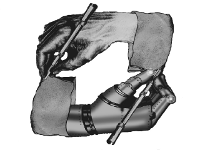
\includegraphics[width=35pt]{figures/lacam}}
\date{19th December 2017 - Université Paris Sud}


{
  \setbeamertemplate{headline}{}
  \setbeamertemplate{footline}{}
  \begin{frame}
    \titlepage
  \end{frame}
}

\begin{frame}[t]
  \frametitle{Outline}
  \footnotesize

  A couple recent topics from my research as a PhD.\par
  A little excursus on  
   \highlighttext[tomato4]{\emph{\textbf{bridging deep and probabilistic models}}} to leverage both
    exact and efficient probabilistic inference and rich and
    compositional representations
   \highlighttext[bgrey2]{\textbf{\emph{towards automating density
         estimation}}} over \highlighttext[peas4]{\emph{\textbf{hybrid domains}}}.\par\bigskip


  Focusing on \emph{\textbf{Sum-Product Networks}}
  (\textbf{SPNs})~\emph{\parencite{Poon2011}} as they can be pivotal for both.
  Talking about \textbf{what} SPNs can offer,
  \textbf{how} they can be exploited and \textbf{why} you may want to use them.\par\bigskip

  
  \highlighttext[tomato2]{\textbf{Density estimation} >}\par
  \hspace{20pt} \highlighttext[tomato2]{\textbf{Tractable Probabilistic Models} >}\par
  \hspace{40pt} \highlighttext[tomato3]{\textbf{Sum-Product Networks} >}\par
  \hspace{60pt} \highlighttext[bgrey2]{\textbf{Sum-Product
      Autoencoding} >}\par
  \hspace{80pt} \highlighttext[bgrey4]{\textbf{Automating density estimation} >}\par
  \hspace{100pt} \highlighttext[peas2]{\textbf{Mixed Sum-Product Networks} >} \par
  \hspace{120pt} \highlighttext[peas4]{\textbf{Exploiting MSPNs} >}\par
  \par\bigskip

  
\end{frame}


\begin{frame}[t]
  % \frametitle{\highlighttext[tomato1]{Density estimation}}
  \frametitle{\highlighttext[tomato4]{Learn \emph{once}, exploit \emph{more than once}}}
  \footnotesize
  
   The challenges in the arms race to \emph{\textbf{deeply
       make sense of data}}
   lie into the  ability to effectively make use of \highlighttext[tomato0]{\emph{\textbf{unlabeled data}}}
   and to efficiently reason about it, i.e. to make
   \emph{\textbf{inference}} about their configurations and
   relationships\par
   \hfill\begin{minipage}{1.0\linewidth}
    \vspace{5pt}
    \raggedleft
    $\color{violet}\boldsymbol\Rightarrow$
    \scriptsize
    e.g., \it
    how to understand the flow of traffic in a city from historical
    records,\par
    traffic light sensors and camera recordings?
    %how to understand\par why congestions happen and how to predict the next ones?
  \end{minipage}\par\bigskip

   \emph{\textbf{Density estimation}} is the unsupervised task of
    learning an estimator for the joint probability distribution
    $p(\mathbf{X})$ from i.i.d. samples $\mathcal{D}=\{\mathbf
    x^i\}_{i=1}^m$ over random variables (RVs) $\mathbf{X}$
    Given such an estimator, answer a wide range of probabilistic
    queries:\par
    \hfill\begin{minipage}{0.75\linewidth}
    \vspace{5pt}
    \raggedleft
    $\color{violet}\boldsymbol\Rightarrow$
    \scriptsize
    e.g., \emph{complete evidence} (EVA), \emph{marginals} (MAR), \emph{conditionals} (CON),\par
    \emph{Most Probable Explanaition} (MPE) and MAP \emph{assignments},\dots%\par
    %\emph{partition function} ($Z$), \emph{sampling} (SAM), \dots
  \end{minipage}\par\bigskip

    \highlighttext[tomato0]{\textbf{\emph{Learn once, exploit it several times}}} philosophy to
  density estimation: learn one \emph{tractable} probabilistic model
  in an unsupervised way from data, \emph{then}:
  \begin{itemize}
    \setlength{\itemsep}{0pt}
  \item perform (several kinds of) \emph{\textbf{inference ad
        libitum}}
    \item \emph{\textbf{exploit it for predictive tasks}} later, without training again
  \end{itemize}



\end{frame}

\begin{frame}[t]
  \frametitle{\highlighttext[bgrey2]{The density estimation pipeline}}
  \footnotesize
  
  \begin{enumerate}
    \setlength{\itemindent}{0pt}
  \item decide a \textbf{parametric form} for the estimator
    \begin{itemize}
      \setlength{\itemindent}{-10pt}
      \scriptsize
    \item  a parametric form for individual RVs \hfill{% $\color{violet}\boldsymbol\Rightarrow$
    \scriptsize \emph{\color{bgrey4}(e.g., are counts of vehicles poisson distributed?)}}
\item the dependency structure parametric form\hfill{
    \scriptsize \emph{\color{bgrey4}(e.g., are jams influenced by
      salary growth?)}}
    \end{itemize}
  \item \textbf{fit the estimator} to the data \hfill{
        \scriptsize \emph{\color{bgrey4}(e.g., optimize data likelihood)}}
    \begin{itemize}
      \setlength{\itemindent}{-10pt}
      \scriptsize
    \item fit model structure 
      \item fit model parameters
    \end{itemize}
  \item perform \textbf{inference \emph{ad libitum}}
    \begin{itemize}\scriptsize
      \setlength{\itemindent}{-10pt}
    \item several kinds of probabilistic queries \hfill{
    \scriptsize \emph{\color{bgrey4}(e.g., how likely is to see ?)}}
    \item compute statistics, metrics, descriptors\hfill{
        \scriptsize \emph{\color{bgrey4}(e.g., mutual information)}}
      \item make sense of the data and the model (\textbf{interpretability})\hfill{
        \scriptsize \emph{\color{bgrey4}(e.g., what has been learned?)}}
      \item\dots
    \end{itemize}
  

    \item \textbf{(\emph{re-})use knowledge} in other tasks \hfill\begin{minipage}{0.57\linewidth}
  \vspace{10pt}
      \raggedleft
      \scriptsize \emph{\color{bgrey4}(e.g., can representations
          learned for traffic counts be used to predict where to build
          a city mall?)}
\end{minipage}%  \hfill\begin{minipage}{0.5\linewidth}{
  \end{enumerate}
\end{frame}


\begin{frame}[t]
  \frametitle{\highlighttext[tomato2]{Tractable Probabilistic Models (TPMs)}}
  \footnotesize

    Classical Probabilistic Graphical Models (PGMs) like \emph{\textbf{Bayesian Networks}}
    (\textbf{BNs}) and \emph{\textbf{Markov Networks}} (\textbf{MNs}) are highly expressive but
    exact inference is in general \emph{NP-hard}.\par\bigskip
    % \vspace{20pt}

    \emph{\textbf{Tractable Probabilistic Models} }  (\textbf{TPMs})
     are density estimators for which some kind of  
     {\color{tractable_green}\textbf{inference is}
    \textbf{\emph{exact}}  and \textbf{\emph{tractable}}}
  , i.e. \emph{polynomial} in the number
    of RVs:
    \hspace{20pt}\begin{minipage}{1.0\columnwidth}
      \vspace{2pt}
      \scriptsize
    \raggedleft
    $\rightarrow$
    e.g., \highlighttext[petroil2]{\emph{\textbf{bounded tree-width PGMs}}}, \highlighttext[gold2]{\emph{\textbf{computational graphs}}} and \highlighttext[lacamdarklilac5]{\emph{\textbf{neural autoregressive models}}}
  \end{minipage}
  \par\bigskip\vspace{5pt}

   \begin{minipage}[t]{0.19\linewidth}
      \begin{center}
        \highlighttext[petroil2]{\scriptsize\textbf{BN trees}}% ~\customcite{Meila2000}
        \\[5pt]
        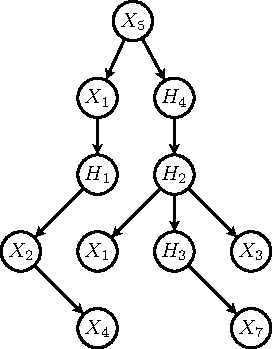
\includegraphics[width=0.8\linewidth]{figures/tree}\\
        \begin{minipage}[t]{0.87\linewidth}
          \tiny \flushleft 
          \textcolor{tractable_green}{\cmark \textbf{EVI}}, \textcolor{tractable_green}{\cmark \textbf{SAM}},
          \textcolor{tractable_green}{\cmark \textbf{MAR}},\par
          \textcolor{tractable_green}{\cmark \textbf{CON}},
          \textcolor{tractable_green}{\cmark \textbf{MPE}},
          \textcolor{tractable_green}{\cmark \textbf{Z}}
        \end{minipage}
      \end{center}
    \end{minipage}\begin{minipage}[t]{0.19\linewidth}
      \begin{center}
        \highlighttext[gold2]{\scriptsize\textbf{d-DNNFs}}% ~\customcite{Darwiche2009}
        \\[5pt]
        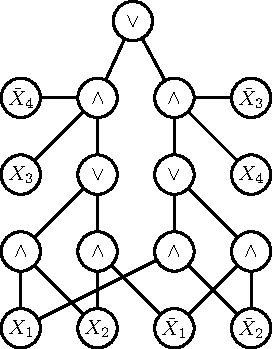
\includegraphics[width=0.8\linewidth]{figures/ddnnf}\\
        \begin{minipage}[t]{0.87\linewidth}
          \tiny \flushleft
          \textcolor{tractable_green}{\cmark \textbf{EVI}}, \textcolor{untractable_red}{\xmark \textbf{SAM}},
          \textcolor{tractable_green}{\cmark \textbf{MAR}},\par
          \textcolor{tractable_green}{\cmark \textbf{CON}},
          \textcolor{tractable_green}{\cmark \textbf{MPE}},
          \textcolor{tractable_green}{\cmark \textbf{Z}}
        \end{minipage}
      \end{center}
    \end{minipage}\begin{minipage}[t]{0.23\linewidth}
      \begin{center}
        \highlighttext[gold2]{\scriptsize\textbf{SPNs}}% ~\customcite{Poon2011}
        \\[5pt]
        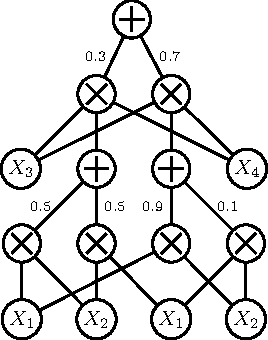
\includegraphics[width=0.7\linewidth]{figures/spn}\\
        \begin{minipage}[t]{0.83\linewidth}
          \tiny \flushleft
          \textcolor{tractable_green}{\cmark \textbf{EVI}}, \textcolor{tractable_green}{\cmark \textbf{SAM}},
          \textcolor{tractable_green}{\cmark \textbf{MAR}},\par
          \textcolor{tractable_green}{\cmark \textbf{CON}},
          \textcolor{untractable_red}{\xmark \textbf{MPE}},
          \textcolor{tractable_green}{\cmark \textbf{Z}}
        \end{minipage}
      \end{center}
    \end{minipage}\begin{minipage}[t]{0.19\linewidth}
      \begin{center}
        \highlighttext[lacamdarklilac5]{\scriptsize\textbf{NADEs}}% ~\customcite{Larochelle2011}
        \\[5pt]
        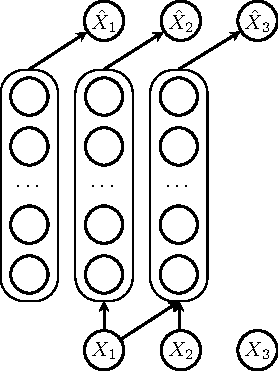
\includegraphics[width=0.79\linewidth]{figures/nade}\\
        \begin{minipage}[t]{0.87\linewidth}
          \tiny \flushleft
          \textcolor{tractable_green}{\cmark \textbf{EVI}}, \textcolor{tractable_green}{\cmark \textbf{SAM}},
          \textcolor{untractable_red}{\xmark \textbf{MAR}},\par
          \textcolor{untractable_red}{\xmark \textbf{CON}},
          \textcolor{untractable_red}{\xmark \textbf{MPE}},
          \textcolor{tractable_green}{\xmark \textbf{Z}}
        \end{minipage}
      \end{center}
    \end{minipage}\begin{minipage}[t]{0.19\linewidth}
       \begin{center}
         \highlighttext[lacamdarklilac5]{\scriptsize\textbf{MADEs}}% ~\customcite{Germain2015}
         \\[5pt]
         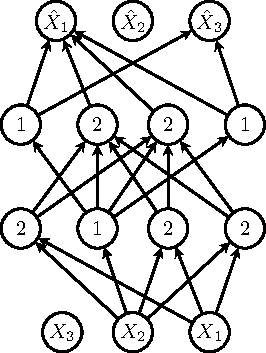
\includegraphics[width=0.79\linewidth]{figures/made}\\
         \begin{minipage}[t]{0.87\linewidth}
           \tiny \flushleft
           \textcolor{tractable_green}{\cmark \textbf{EVI}}, \textcolor{tractable_green}{\cmark \textbf{SAM}},
           \textcolor{untractable_red}{\xmark \textbf{MAR}},\par
           \textcolor{untractable_red}{\xmark \textbf{CON}},
           \textcolor{untractable_red}{\xmark \textbf{MPE}},
           \textcolor{tractable_green}{\xmark \textbf{Z}}
         \end{minipage}
      \end{center}
    \end{minipage}
\end{frame}







  \begin{frame}[t]
    \frametitle{\highlighttext[tomato3]{Sum-Product Networks (SPNs)}}
    \footnotesize
      A \emph{Sum-Product Network} $S$ over RVs $\mathbf X$ is defined via
  rooted weighted DAG consisting of
  distribution \highlighttext[purple]{\emph{\textbf{leaves}}} (network inputs),  \highlighttext[gold2]{\emph{\textbf{sum}}} and \highlighttext[petroil2]{\emph{\textbf{product}}}
  nodes (inner nodes).

  \vspace{0.5 cm}

  Each sub-network $S_{n}$ defines an unnormalized probability
  distribution over the subset of RVs appearing in it, $\mathsf{sc}(n)\subseteq\mathbf X$.\par\bigskip
\begin{minipage}{0.63\textwidth}
\begin{itemize}
\item  A % \emph{\color{purple}\textbf{leaf}}
  leaf
  $n$ defines a \textbf{tractable distribution}\par

  \hfill ${\color{purple}\phi_{n}(\mathbf{x})}= p(\mathbf{x}_{|\mathsf{sc}(n)})$
\item a % \emph{\color{petroil2}\textbf{product node}}
  product node
      $n$ represents a \textbf{factorization over independent
        components}\par
      \hfill${\color{petroil2}S_{n}(\mathbf{x})}=\prod_{c\in \mathsf{ch}(n)}S_{c}(\mathbf{x})$

  
\item a % \emph{\color{gold2}\textbf{sum node}}
  sum node
    $n$  denotes a
    \textbf{mixture} over its children distributions% , summing out a
    % \emph{\textbf{latent RV}} (\textbf{LV})
    \par
    %$\highlight[gold2]{S_{n}(\mathbf{x})=\sum_{c\in
    %\mathsf{ch}(n)}w_{nc}S_{c}(\mathbf{x})}$
    \hfill ${\color{gold2}S_{n}(\mathbf{x})}=\sum_{c\in \mathsf{ch}(n)}w_{nc}S_{c}(\mathbf{x})$
\end{itemize}


\end{minipage}\hspace{15pt}
\begin{minipage}{0.28\textwidth}
  \vspace{-20pt}
\centering
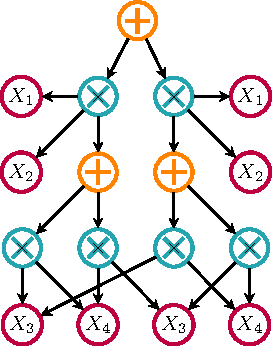
\includegraphics[width=0.85\columnwidth]{figures/spn-colored}
\end{minipage}

  \end{frame}


  \begin{frame}[t]
    \frametitle{\highlighttext[tomato3]{SPNs: exact and tractable inferences}}
    \footnotesize
    \vspace{5pt}
    Let $\nodeset{S}^{\oplus}$ (resp. $\nodeset{S}^{\otimes}$) be the set of all sum
    (resp. product) nodes in an SPN $S$, then 
\begin{itemize}  
\item    $S$ is \highlighttext[tomato0]{\emph{\textbf{complete}}} iff $\forall n\in
  \nodeset{S}^{\oplus},\forall c_{1}, c_{2}\in \mathsf{ch}(n):
  \mathsf{sc}(c_{1})=\mathsf{sc}(c_{2})$
\item    $S$ is \highlighttext[tomato0]{\emph{\textbf{decomposable}}} iff $\forall n\in
  \nodeset{S}^{\otimes},\forall c_{1}, c_{2}\in \mathsf{ch}(n)% , c_{1}\neq c_{2}
  :
  \mathsf{sc}(c_{1})\cap\mathsf{sc}(c_{2})=\emptyset$
\end{itemize}\par\bigskip

If $S$ is complete and decomposable, then it is
\highlighttext[tomato0]{\emph{\textbf{valid}}} and allows for the
efficient computation of a network polynomial:
\begin{minipage}{1.0\linewidth}
      \vspace{-10pt}
      \raggedleft
      $\color{violet}\boldsymbol\Rightarrow$    
% \hfill$\rightarrow$
\emph{\textbf{evidence}, \textbf{marginals}, \textbf{Z}} in time
linear to $|S|$
\end{minipage}\customcite{Darwiche2009,}\customcite{Poon2011}\par\bigskip

An SPN $S$ is 
\highlighttext[tomato0]{\textbf{\emph{selective}}}~\customcite{Peharz2014b}, iff $\forall \mathbf{x}^{i}\sim\mathbf{X},\forall
n\in\nodeset{S}^{\oplus}\colon
|\{c \cbar c\in\mathsf{ch}(n):S_{c}(\mathbf{x}^{i})>0\}|
\leq 1$\par
% \hfill$\rightarrow$
\begin{minipage}{1.0\linewidth}
  \vspace{2pt}
      \raggedleft
      $\color{violet}\boldsymbol\Rightarrow$
\emph{\textbf{MPE inference}, \textbf{assignments}} in time
linear to $|S|$
\end{minipage}\customcite{Choi2017}\par\bigskip

  \end{frame}

\begin{frame}[t]
  \frametitle{\highlighttext[tomato3]{Building SPNs\dots}}
  \footnotesize
  \onslide<1-4>{\begin{minipage}[t]{0.3\linewidth}
      \begin{center}
        \only<1>{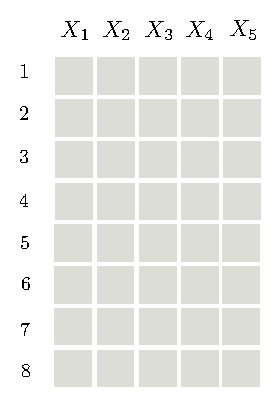
\includegraphics[width=0.648\linewidth]{figures/grid-0}}
        \only<2-4>{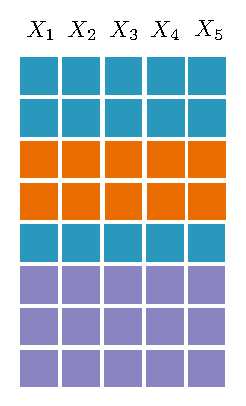
\includegraphics[width=0.5791\linewidth]{figures/grid-1}}
      \end{center}
    \end{minipage}}\hspace{10pt}\onslide<3-4>{\begin{minipage}[t]{0.3\linewidth}
      \begin{center}
        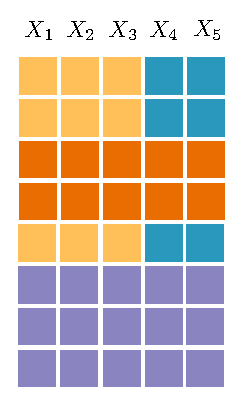
\includegraphics[width=0.5832\linewidth]{figures/grid-2}
      \end{center}
    \end{minipage}}\hspace{10pt}\onslide<4>{\begin{minipage}[t]{0.3\linewidth}
      \begin{center}
        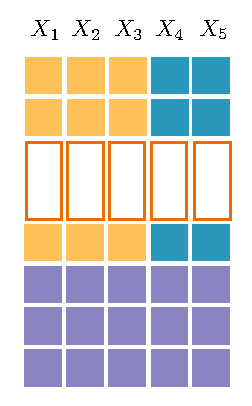
\includegraphics[width=0.59535\linewidth]{figures/grid-3}
      \end{center}
    \end{minipage}}\\
  \vspace{5pt}
  \onslide<2-4>{\raisebox{0pt}{\begin{minipage}[t]{0.3\linewidth}
        \begin{center}
          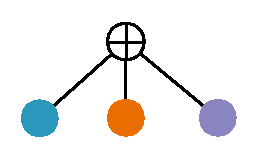
\includegraphics[width=0.5791\linewidth]{figures/learnspn-1}
        \end{center}
      \end{minipage}}}\hspace{6pt}\onslide<3-4>{\raisebox{-20pt}{\begin{minipage}[t]{0.3\linewidth}
        \begin{center}
          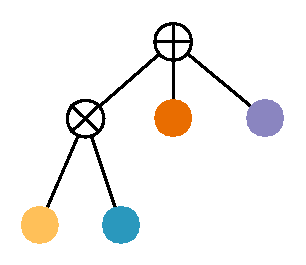
\includegraphics[width=0.6723\linewidth]{figures/learnspn-2}
        \end{center}
      \end{minipage}}}\hspace{5pt}\onslide<4>{\raisebox{-18pt}{\begin{minipage}[t]{0.3\linewidth}
        \begin{center}
          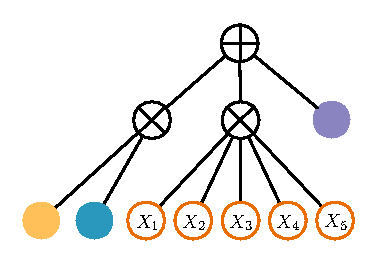
\includegraphics[width=0.81\linewidth]{figures/learnspn-3}
        \end{center}
      \end{minipage}}}\par\bigskip
  \only<1>{Learning both structure and parameters of SPNs with
    algorithmic variants of \textbf{LearnSPN}}
  \only<2>{Looking for sub-population in the data---\highlighttext[tomato0]{\emph{\textbf{clustering}}}---to
    introduce sum nodes\dots}
  \only<3>{\dots seeking \highlighttext[tomato0]{\emph{\textbf{statistical independence}}} among RVs to factorize into product
  nodes}
  \only<4>{\dots learning smaller estimators as a \textbf{\emph{a recursive data crawler}}}
 \customcitenomark{Vergari2015}\customcitenomark{Gens2013}
\end{frame}

  
\begin{frame}[t]
    \frametitle{\highlighttext[tomato3]{\dots and building upon SPNs}}
    \footnotesize
    
    SPNs as \emph{\textbf{recursive hierarchical decomposition}} of larger models into smaller
    ones.\par
    Tackling inference and learning complexity by pushing it down
    towards the leaves\par
    \begin{minipage}{1.0\linewidth}
  \vspace{2pt}
      \raggedleft
      $\color{violet}\boldsymbol\Rightarrow$
      \scriptsize
 computing \highlighttext[tomato0]{\emph{\textbf{mode}}}, mean, variance,\dots efficiently
\end{minipage}~\customcite{Vergari2016a}\par
    \begin{minipage}{1.0\linewidth}
  \vspace{2pt}
      \raggedleft
      $\color{violet}\boldsymbol\Rightarrow$
      \scriptsize
 \highlighttext[tomato0]{\emph{\textbf{delegating encoding and decoding}}} to leaf distributions
\end{minipage}~\customcite{Vergari2017}\par\bigskip
    The Sum-Product Theorem~\customcite{Friesen2016} hints at generalizations
    over other semi-rings\par
    \begin{minipage}{1.0\linewidth}
  \vspace{2pt}
      \raggedleft
      $\color{violet}\boldsymbol\Rightarrow$
      \scriptsize
 e.g., composing kernel machines
\end{minipage}~\customcite{Gens2017}\par\bigskip

    SPNs as \textbf{divide-et-impera} machines
 \textbf{\emph{gluing and orchestrating inference}} among
 different (possibly heterogeneous) models.\par
 \begin{minipage}{1.0\linewidth}
  \vspace{2pt}
      \raggedleft
      $\color{violet}\boldsymbol\Rightarrow$
      \scriptsize
 performing \highlighttext[tomato0]{\emph{\textbf{MPE inference over autoencoders}}} from different domains
\end{minipage}~\customcite{Molina2017b}
  \end{frame}


\begin{frame}[t]
    \frametitle{\highlighttext[tomato4]{Exploiting SPNs \emph{more than once}}}
    \footnotesize
    
    Learn one SPN $S$ generatively from data
    $\{\mathbf{x}^{i}\sim\mathbf{X}\}_{i=1}^{m}$ to estimate
    $p(\mathbf{X})$ and then exploit it---\emph{without
    retraining} it---by \highlighttext[tomato0]{\textbf{\emph{interpreting it as a neural network}}}:
    \begin{itemize}
    \item as a \textbf{feature extractor} for Representation Learning (RL)\par
      \begin{minipage}{1.0\linewidth}
 %     \vspace{2pt}
      \raggedleft
      $\color{violet}\boldsymbol\Rightarrow$
      \scriptsize
     \emph{sum, product nodes or scope aggregations as filters}
      \end{minipage}~\customcite{Vergari2016a}
\item as an \highlighttext[tomato0]{\emph{\textbf{autoencoder}}} mapping back and forth embeddings\par
  \begin{minipage}{1.0\linewidth}
%  \vspace{2pt}
      \raggedleft
      $\color{violet}\boldsymbol\Rightarrow$
      \scriptsize
 \emph{Sum-Product Autoencoding}
\end{minipage}~\customcite{Vergari2017}
\item understanding learned representations\par
  \begin{minipage}{1.0\linewidth}
%  \vspace{2pt}
      \raggedleft
      $\color{violet}\boldsymbol\Rightarrow$
      \scriptsize
 \emph{visualizing filters in the input space}
\end{minipage}% ~\customcite{Vergari2016a}
    \end{itemize}\par\bigskip

    Moreover the interpretation of SPNs as NNs enables
    \begin{itemize}
      \setlength{\itemsep}{0pt}
    % \item extracting embeddings as neuron activations
    \item efficient implementations running on GPUs
    \item structure learning as a constrained optimization problem
      
    \end{itemize}
       
\end{frame}
  
\begin{frame}[t]
    \frametitle{\highlighttext[tomato3]{MPE inference with SPNs}}
    \footnotesize
    Exact \emph{\textbf{MPE inference}}, e.g. computing for RVs
    $\mathbf{Q},\mathbf{O}\subset\mathbf{X}$,
    $\mathbf{Q}\cup\mathbf{O}=\mathbf{X}$, 
    $\mathbf{Q}\cap\mathbf{O}=\emptyset$
    $$\argmax\nolimits_{\mathbf{q}\sim\mathbf{Q}}p(\mathbf{q}|\mathbf{O})$$
    
    is NP-hard for a general
 SPN $S$ over $\mathbf{X}$ but can be approximated in linear
 time in $|S|$
 by the $\mathsf{MaxProdMPE}$ algorithm (but exact for selective
 SPNs)\par\bigskip
 \onslide<2-4>{\begin{minipage}[t]{0.4\linewidth}
     \vspace{-100pt}
      \begin{center}
        \only<2>{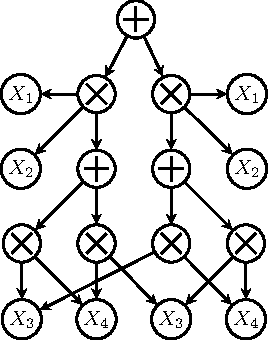
\includegraphics[width=0.6\linewidth]{figures/mpn-eval-i}}
        \only<3>{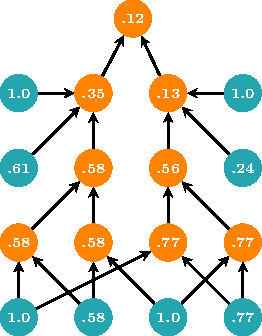
\includegraphics[width=0.6\linewidth]{figures/mpn-eval-ii}}
        \only<4>{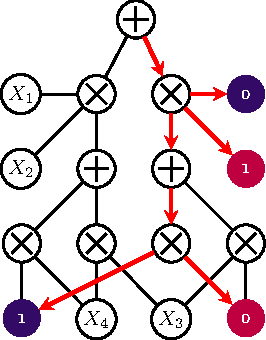
\includegraphics[width=0.6\linewidth]{figures/mpn-eval-iii}}
      \end{center}
    \end{minipage}}\onslide<2-4>{\raisebox{100pt}{\begin{minipage}[t]{0.6\linewidth}
        \vspace{0pt}
        \only<2>{E.g. to compute the MPE state of RVs
          $\mathbf{Q}=\{X_{1},X_{3}\}$ given $\mathbf{O}=\{X_{2},X_{4}\}$
          $$\argmax\nolimits_{\mathbf{q}\sim\mathbf{Q}}p_{S}(\mathbf{q},X_{2}=1,X_{4}=0),$$
        $\mathsf{MaxProdMPE}$ first turns $S$ into a \highlighttext[tomato0]{\emph{\textbf{Max-Product
     Network}} (\textbf{MPN})}  $M$, by replacing sum nodes with \emph{max
 nodes} and leaf distributions with \emph{maximizing distributions}}
        \only<3>{\dots then $M$ is evaluated \highlighttext[tomato0]{\emph{\textbf{bottom-up}}} to
          compute $M(\mathbf{O})$
 by propagating evidence from children to parents and marginalizing
 over query RVs $\mathbf{Q}$}
\only<4>{A Viterbi-style step
retrieves the query assignments to $\mathbf{Q}$ \highlighttext[tomato0]{\emph{\textbf{growing a tree
      path}} \textbf{top-down}}, starting from the root:
\begin{itemize}
\item following only the maximum activation children for a max node
\item following all child branches for product nodes
  \item maximizing on leaf distributions over $\mathbf{Q}$
\end{itemize}}
\end{minipage}}}
  
 \customcitenomark{Poon2011}\customcitenomark{Vergari2017}    
\end{frame}
  

\begin{frame}[t]
  \frametitle{\highlighttext[bgrey0]{Sum-Product Autoencoding (SPAE)}}
  \footnotesize

  Given an SPN $S$---\emph{\textbf{unsupervisedly learned}} to
  estimate $p(\mathbf{X})$ we want to {{\textbf{\emph{encode}}}} a sample
  $\mathbf{x}^{i}\sim\mathbf{X}$ as an \emph{embedding} $\mathbf{e}^{i}$ in a new $d$-dimensional
space $\mathbf{E}_{\mathbf{X}}\subseteq\mathbb{R}^{d}$
    $$\mathbf{e}^{i} = f_{S}(\mathbf{x}^{i}).$$

 For \textbf{\emph{decoding}}, on the other hand, we seek an inverse function
$g\colon\mathbf{E}_{\mathbf{X}}\rightarrow\mathbf{X}$ such that
$$ g_{S}(\mathbf{e}^{i}) =
{\tilde{\mathbf{x}}}^{i}\approx{{\mathbf{x}}}^{i}.$$

Embeddings over $\mathbf{X}$ can be later used in {\textbf{\emph{predictive
  tasks}}} as features
\begin{minipage}{1.0\linewidth}
 %     \vspace{2pt}
      \raggedleft
      $\color{violet}\boldsymbol\Rightarrow$
      \scriptsize
     \emph{e.g. \highlighttext[tomato0]{\emph{\textbf{to predict}}} a RV $Y$% :
     }
\end{minipage}\\[5pt]
or as the output of a predictive model $p$ whose target space
is $\mathbf{E}_{\mathbf{X}}$
\begin{minipage}{1.0\linewidth}
 %     \vspace{2pt}
      \raggedleft
      $\color{violet}\boldsymbol\Rightarrow$
      \scriptsize
     \emph{e.g. \highlighttext[tomato0]{\emph{\textbf{to disentangle}}} label dependencies $\mathbf{Y}$ in MLC% : {\scriptsize${\quad(\mathbf{X}\xRightarrow{\scriptscriptstyle
             % p}(\mathbf{Y}\xrightarrow{\scriptscriptstyle
             % f_{S}}\mathbf{E}_{\mathbf{Y}}))\xrightarrow{\scriptscriptstyle
             % g_{S}}\mathbf{Y}}$}
     }
\end{minipage}\par\bigskip

We equip $S$ with $f_{S}$ and $g_{S}$ by exploiting MPE inference routines
\begin{minipage}{1.0\linewidth}
  \vspace{5pt}
  \raggedleft
  $\color{violet}\boldsymbol\Rightarrow$
      {\scriptsize
     \emph{dealing with categorical and continuous representations}}\par
      $\color{violet}\boldsymbol\Rightarrow$
      {\scriptsize
     \emph{dealing with \highlighttext[tomato0]{\emph{\textbf{partial embeddings}}}}}
   \end{minipage}\par\bigskip

\end{frame}

   

\begin{frame}[t]
    \frametitle{\highlighttext[bgrey1]{$\mathsf{CAT}$ embeddings (I)}}
    \footnotesize

    Given an SPN $S$ over $\mathbf{X}$,  to each sum node
    $n\in\nodeset{S}^{\oplus}$ is associated a \emph{\textbf{categorical latent
    variable}} (\textbf{LV}) $Z_{n}$
    having values $z_{n}\in\{0,\dots,|\mathsf{ch}(n)|-1\}$.\par\bigskip

    It would be natural to encode $\mathbf{x}^{i}$ through
    the  LVs in $S$,
    i.e. $\mathbf{E}_{\mathbf{X}}=\mathbf{Z}_{S}$ ($d=|\nodeset{S}^{\oplus}|$):
\begin{equation}
  \label{eq:lv-enc}
  f_{S}(\mathbf{x}^{i}) 
  = f_{\mathsf{CAT}}(\mathbf{x}^{i}) \triangleq \tilde{\mathbf{z}}^{i} = \argmax\nolimits_{\mathbf{z}^i}p(\mathbf{z}^i \cbar \mathbf{x}^{i}),
\end{equation}
i.e. $\mathbf{x}^{i}$ is encoded as the \emph{categorical} vector
$\tilde{\mathbf{z}}^{i}$ %---also explaining the name of the embeddings: {\bf CAT}egorial---
comprising the \highlighttext[tomato0]{\emph{\textbf{MPE state}}} for $\mathbf{Z}_{S}$.\par\bigskip

Analogously, the decoding of $\tilde{\mathbf{z}}^{i}$
 through $g_{S}$ can be defined as:

\begin{equation}
  \label{eq:lv-dec}
  g_{S}(\tilde{\mathbf{z}}^{i}) 
  = g_{\mathsf{CAT}}(\tilde{\mathbf{z}}^{i}) \triangleq \tilde{\mathbf{x}}^{i} = \argmax\nolimits_{\mathbf{x}^i} p(\mathbf{x}^i \cbar \tilde{\mathbf{z}}^{i}).
\end{equation}\\[10pt]

However, this requires performing MPE inference over the \highlighttext[tomato0]{\emph{\textbf{joint
probability distribution}}} over $\mathbf{V}=(\mathbf{X}, \mathbf{Z}_{S})$

\begin{minipage}{1.0\linewidth}
 %     \vspace{2pt}
      \raggedleft
      $\color{violet}\boldsymbol\Rightarrow$
      \scriptsize
     \emph{we need to deal with an \emph{\textbf{augmented
           SPN}}~\customcite{Peharz2016} $\overline{S}$ over $\mathbf{V}$}
\end{minipage}
\end{frame}

\begin{frame}[t]
    \frametitle{\highlighttext[bgrey1]{$\mathsf{CAT}$ embeddings (II)}}
    \footnotesize

    \begin{figure}[!ht]
      \vspace{-10pt}
  \raggedright
   %\centering
   % width: width=0.20\columnwidth
   % hspace: 25pt
   \setlength{\tabcolsep}{3pt}
    \begin{tabular}{ccccc}
     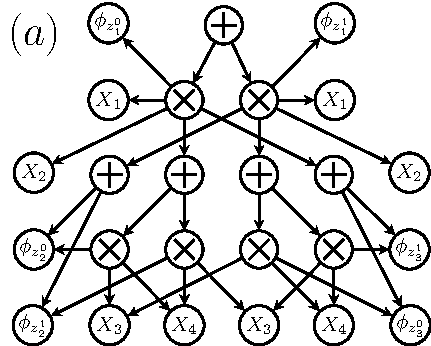
\includegraphics[width=0.17\columnwidth]
     {figures/spn-mpe-aug-eval-i} \label{fig:spn-aug-eval-i}&
     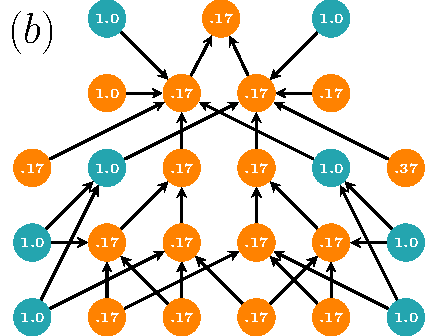
\includegraphics[width=0.17\columnwidth]
     {figures/spn-mpe-aug-eval-ii} \label{fig:spn-aug-eval-ii}&
     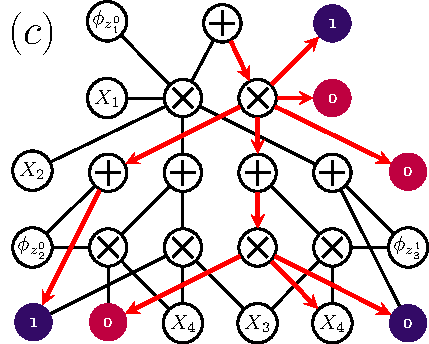
\includegraphics[width=0.17\columnwidth]
     {figures/spn-mpe-aug-eval-iii} \label{fig:spn-aug-eval-iii}&
     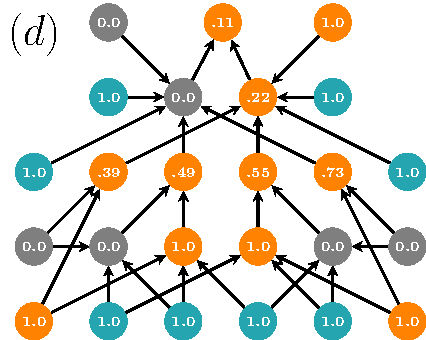
\includegraphics[width=0.17\columnwidth]
     {figures/spn-mpe-aug-eval-iiii} \label{fig:spn-aug-eval-iiii}&
     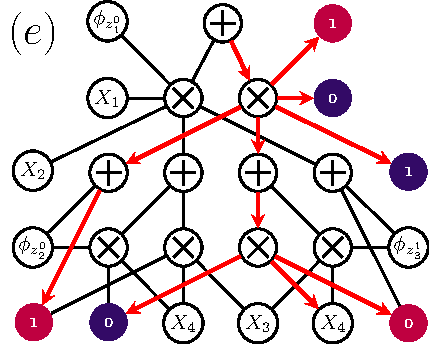
\includegraphics[width=0.17\columnwidth]
     {figures/spn-mpe-aug-eval-v} \label{fig:spn-aug-eval-v}
     %(a) & (b) & (c) & (d) & (e)
    \end{tabular}
 \end{figure}

    To solve both Eq.~\eqref{eq:lv-enc} and Eq.~\eqref{eq:lv-dec}, 
has to be run
$\mathsf{MaxProdMPE}$ twice on the augmented MPN $\overline{M}$.
Since each application of $\mathsf{MaxProdMPE}$ involves a bottom-up and a backtracking pass, we need in total 4 passes over $\overline{M}$.
\begin{minipage}{1.0\linewidth}
 %     \vspace{2pt}
      \raggedleft
      $\color{violet}\boldsymbol\Rightarrow$
      \scriptsize
     \emph{$\overline{M}$ is selective, hence MPE inference is exact!}
\end{minipage}\par\bigskip
    

Materializing $\overline{M}$ scales quadratically, thus we directly use $M$, evaluating $M(\mathbf{x}^{i})$ in a bottom-up
pass once and then \highlighttext[tomato0]{\emph{\textbf{growing a tree path}}} $\theta$ while collecting the states:
\begin{equation}
  \label{eq:cat-appr}
  z_{j}^{i} = \argmax\nolimits_{k\in\{0, \dots, |\mathsf{ch}(n_j)|\}}w_{n_{j}c_{k}}M_{c_{k}}(\mathbf{x}^{i}),
\end{equation}
for each $Z_{j}\in\mathbf{Z}^{{\theta}}_{S}$, where
$\mathbf{Z}^{{\theta}}_{S}$ are the LVs associated only to the max nodes in
$\theta$.
\begin{minipage}{1.0\linewidth}
 %     \vspace{2pt}
      \raggedleft
      $\color{violet}\boldsymbol\Rightarrow$
      \scriptsize
     \emph{$\mathsf{CAT}$ embeddings are very \highlighttext[tomato0]{\emph{\textbf{sparse}}}!}
\end{minipage}   
\end{frame}

\begin{frame}[t]
  \frametitle{\highlighttext[bgrey1]{$\mathsf{CAT}$ embeddings (III)}}
  \footnotesize
  $\mathsf{CAT}$ embeddings are \highlighttext[tomato0]{\textbf{\emph{compact} and \emph{linear}
  representations of trees \emph{{}}}}, the \textbf{induced trees} in $S$~\customcite{Zhao2015}.\par\bigskip

  % 
We can interpret the semantics of $\mathsf{CAT}$ embeddings
by visualizing \highlighttext[tomato0]{\emph{\textbf{the latent factors of variations}}} encoded in $\mathbf{Z}_{S}$ 
through the \emph{clusters} of samples sharing the same
representations~\customcite{Vergari2016a}.

\begin{figure}[!t]
  % \centering
  \raggedright
  %\subfloat[]{
    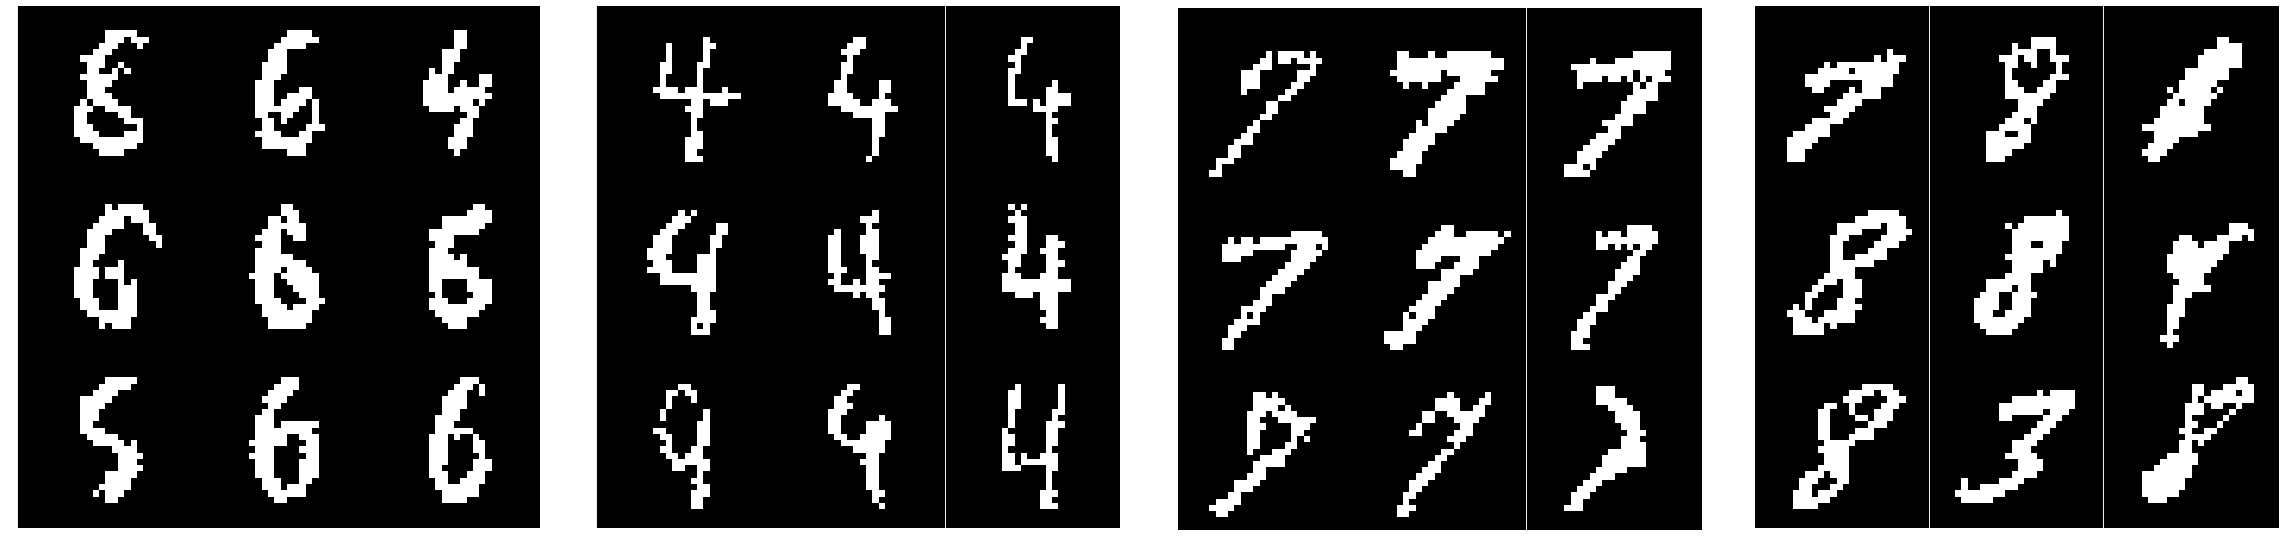
\includegraphics[width=0.75\columnwidth]
    {figures/hid-clu} \label{fig:hid-clu}%}\hspace{6pt}
  \label{fig:bmnist-hid}
\end{figure}
%
%
\vspace{-5pt}
For an SPN learned on MNIST, samples sharing the
same $\mathsf{CAT}$ encoding---even if belonging to different classes, 
clearly 
share \emph{\textbf{stylistic aspects}} like \emph{orientation} and \emph{stroke}.

\end{frame}

\begin{frame}[t]
  \frametitle{\highlighttext[bgrey2]{$\mathsf{ACT}$ embeddings (I)}}
  \footnotesize
SPNs  be interpreted as deep neural networks
with sparse \textbf{\emph{constrained topology}} in which neurons \highlighttext[tomato0]{{\textbf{\emph{labeled}}}} by the scope function $\mathsf{sc}$---enabling a \emph{direct encoding} of the input% ~\cite{Bengio2012}
---retaining a \highlighttext[tomato0]{\emph{\textbf{fully probabilistic
semantics}}}~\customcite{Vergari2016a}.
\begin{minipage}{1.0\linewidth}
 %     \vspace{2pt}
      \raggedleft
      $\color{violet}\boldsymbol\Rightarrow$
      \scriptsize
     \emph{each neuron activation, i.e. $S_{n}(\mathbf{x})$, is a valid probability}
\end{minipage}\par\bigskip

Therefore, neuron \emph{\textbf{$\mathsf{ACT}$ivations}} can be used
as features to build embeddings, 
as it is common practice for neural networks and
autoencoders~\parencite{Rifai2011,Marlin2010}
\begin{minipage}{1.0\linewidth}
 %     \vspace{2pt}
      \raggedleft
      $\color{violet}\boldsymbol\Rightarrow$
      \scriptsize
     \emph{however \highlighttext[tomato0]{\emph{\textbf{representations are not arranged layer-wise}}}!}
\end{minipage}\par\bigskip

Let $\nodeset{N}=\{n_{j}\}_{j=1}^{d}\subseteq\nodeset{M}$
 be a set of nodes
in an MPN $M$, by a \emph{certain criterion}.
A sample $\mathbf{x}^{i}$ is encoded into a $d$-dimensional
\textbf{\emph{continuous}} embedding
$f_{S}(\mathbf{x}^{i}) = \mathbf{e}^{i}\in\mathbf{E}_{\mathbf{X}}\subseteq\mathbb{R}^{d}$
by collecting the activations of nodes in $\nodeset{N}$, i.e.
$$e_{j}^{i}=M_{n_{j}}(\mathbf{x}^{i})$$.

\end{frame}


\begin{frame}[t]
  \frametitle{\highlighttext[bgrey2]{$\mathsf{ACT}$ embeddings (II)}}
  \footnotesize
  We can note how \highlighttext[tomato0]{\textbf{\emph{$\mathsf{ACT}$ embeddings implicitly encode an induced tree}}}: 
node activations $\mathbf{e}^{i}_{M}$ are sufficient to determine
which max node child branch to follow, according to
Eq.~\ref{eq:cat-appr}---recompute each hard decision again.\par\bigskip

Therefore, we can build a decoder $g_{\mathsf{ACT}}$ that \emph{\textbf{mimicks only
the
top-down pass}} of $\mathsf{MaxProdMPE}$: growing the induced tree from
the root by following the max sum node child branches---all product
child nodes are followed as usual.\par\bigskip

Given an SPN $S$ over $\mathbf{X}$---equipped with $(f_{\mathsf{CAT}},
g_{\mathsf{CAT}})$ and $(f_{\mathsf{ACT}}, g_{\mathsf{ACT}})$---and a sample $\mathbf{x}^{i}\sim \mathbf{X}$, 
  it holds
  that:
  \begin{equation}
  g_{\mathsf{ACT}}(f_{\mathsf{ACT}}(\mathbf{x}^{i}))=g_{\mathsf{CAT}}(f_{\mathsf{CAT}}(\mathbf{x}^{i})).\label{eq:cat-act-eq}
\end{equation}
  \begin{minipage}{1.0\linewidth}
     %\vspace{-22pt}
      \raggedleft
      $\color{violet}\boldsymbol\Rightarrow$
      \scriptsize
     \emph{different embeddings, but \highlighttext[tomato0]{\textbf{\emph{equivalent reconstructions}}}!}
   \end{minipage}
\end{frame}


\begin{frame}[t]
  \frametitle{\highlighttext[bgrey2]{$\mathsf{ACT}$ embeddings (III)}}
  \footnotesize
Since $\mathsf{ACT}$ embeddings are points  in
the space induced by a collection of \emph{distributions}, SPN nodes are \highlighttext[tomato0]{\textbf{\emph{part-based filters}}} 
operating over different sub-spaces of RVs.\par\bigskip

For an SPN $S$ we can visualize the filter 
  encoded by sub-network $S_{n}$ rooted at
  node $n$ by \emph{\textbf{computing the
      mode}} of the distribution $p_{S_{n}}$:
  $$\mathbf{x}^{*}_{|\mathsf{sc}(n)} =
  \argmax_{\mathbf{x}}S_{n}(\mathbf{x}_{|\mathsf{sc}(n)};
  \mathbf{w})$$\\[-10pt]
\begin{figure}[!t]
  % \centering
  \raggedright
  %\subfloat[]{
   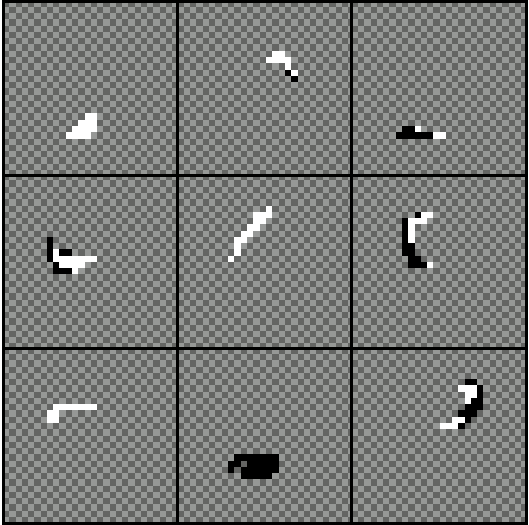
\includegraphics[width=0.18\columnwidth]
    {figures/bmnist-mpe-i} \label{fig:bmnist-mpe-i}\hspace{6pt}
  %\subfloat[]{
    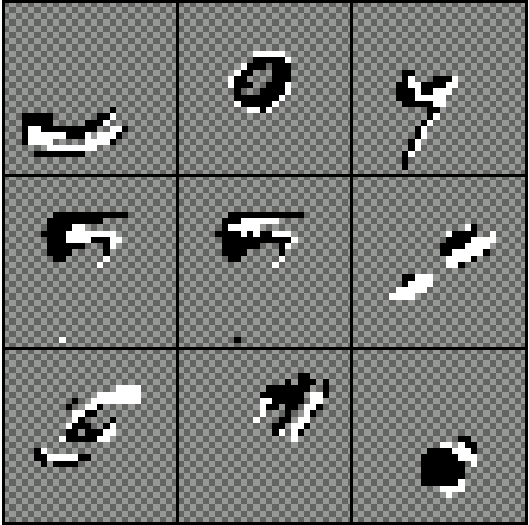
\includegraphics[width=0.18\columnwidth]
    {figures/bmnist-mpe-ii} \label{fig:bmnist-mpe-ii}\hspace{6pt}
  %\subfloat[]{
    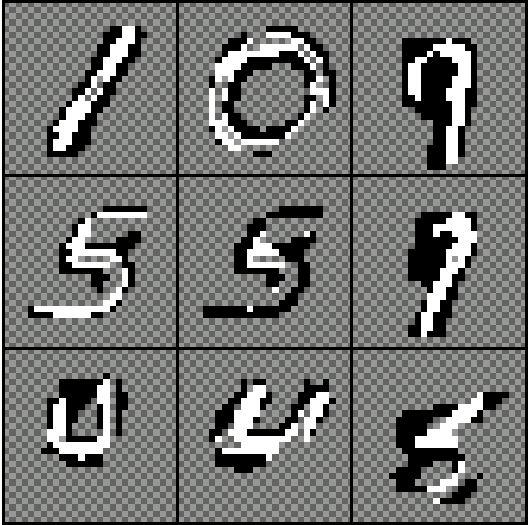
\includegraphics[width=0.18\columnwidth]
    {figures/bmnist-mpe-iii} \label{fig:bmnist-mpe-iii}\hspace{6pt}
  %\subfloat[]{
    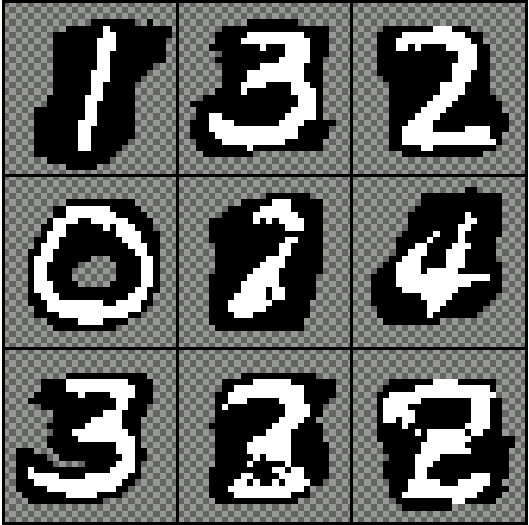
\includegraphics[width=0.18\columnwidth]
    {figures/bmnist-mpe-iiii} \label{fig:bmnist-mpe-iiii}%}

  \end{figure}
E.g., on MNIST, differently complex local patterns emerge
e.g. from small blobs to shape contours and finally full digits\par
\hfill\begin{minipage}{1.0\linewidth}
  \vspace{2pt}
      \raggedleft
      $\color{violet}\boldsymbol\Rightarrow$
a \highlighttext[tomato0]{\emph{\textbf{hierarchy of representations}}}
  structured at levels of abstraction!
\end{minipage}
\end{frame}

\begin{frame}[t]
  \frametitle{\highlighttext[bgrey3]{$\mathsf{CAT}$ vs $\mathsf{ACT}$
    embeddings}}
  \footnotesize
  Even if one can demonstrate that $\mathsf{CAT}$ and $\mathsf{ACT}$
embeddings can lead to the same reconstructions (see
Eq.~\ref{eq:cat-act-eq}), however, \emph{\textbf{they act differently when plugged
in predictive tasks}} (both as feature and target representation spaces).
\begin{minipage}{1.0\linewidth}
 %     \vspace{2pt}
      \raggedleft
      $\color{violet}\boldsymbol\Rightarrow$
      \scriptsize
     \emph{exhaustive empirical evaluation for MLC}
\end{minipage}
\par\bigskip

When employed as features for a predictor (its input)
\highlighttext[tomato0]{\emph{\textbf{$\mathsf{ACT}$ embeddings}}} perform better than $\mathsf{CAT}$ ones
due to their \highlighttext[tomato0]{\emph{\textbf{greater information content}}}.
\begin{minipage}{1.0\linewidth}
     \vspace{7pt}
      \raggedleft
      $\color{violet}\boldsymbol\Rightarrow$
      \scriptsize
     \emph{$\mathsf{CAT}$ embeddings are shared more frequently among samples}
\end{minipage}
\par\bigskip

Conversely, when employed to encode target RVs (a predictor's output)
\highlighttext[tomato0]{\textbf{\emph{classification} for the $\mathsf{CAT}$}
\textbf{\emph{case is easier}}} than \emph{regression} with $\mathsf{ACT}$ embeddings.
\begin{minipage}{1.0\linewidth}
    \vspace{7pt}
      \raggedleft
      $\color{violet}\boldsymbol\Rightarrow$
      \scriptsize
     \emph{simpler prediction task due to the sparsity}
\end{minipage}
\end{frame}


\begin{frame}[t]
  \frametitle{\highlighttext[bgrey4]{Partial embedding decoding}}
  \footnotesize

  Up to now we have considered only \textbf{\emph{fully decodable embeddings}},
i.e. embeddings comprising all the information required to materialize a
\textbf{\emph{complete and well-formed 
tree}} necessary to decode $\mathbf{e}$ into $\tilde{\mathbf{x}}$.\par
%obtain 
%the decoded sample 
%
% real case motivation
In some real cases, however, only incomplete
or \highlighttext[tomato0]{\textbf{\emph{partial embeddings}}} are available: some
values $e_{j}$ are corrupted, invalid or just missing.
\begin{minipage}{1.0\linewidth}
 %     \vspace{2pt}
      \raggedleft
      $\color{violet}\boldsymbol\Rightarrow$
      \scriptsize
     \emph{e.g., data compression}
   \end{minipage}\par\bigskip

SPAE routines offer a natural and efficient way to deal with such
cases: MPE inference.
\begin{minipage}{1.0\linewidth}
 %     \vspace{2pt}
      \raggedleft
      $\color{violet}\boldsymbol\Rightarrow$
      \scriptsize
     \emph{treat \highlighttext[tomato0]{\emph{\textbf{missing embedding components as missing values}}}}
   \end{minipage}\par\bigskip

In practice, if for an $\mathsf{ACT}$ (resp. $\mathsf{CAT}$) embedding
the component $e_{j}^{i}\notin \mathbf{e}^{i}$ (resp. $z_{j}^{i}\notin \mathbf{z}^{i}$) 
corresponds to a node $n_{j}$ activation (resp. LV $Z_{j}$ state),
then it can be imputed
% $\max_{\mathbf{u}\sim
%   \mathsf{sc}(n_{j})}M_{n_{j}}(\mathbf{u})$
% (resp. $\max_{\mathbf{u}\sim
%   \mathsf{sc}(n_{j})}M_{n_{j}}(\mathbf{u})$)
by employing
$\mathsf{MaxProdMPE}$ on the sub-network $M_{n_{j}}$.
\begin{minipage}{1.0\linewidth}
 %     \vspace{2pt}
      \raggedleft
      $\color{violet}\boldsymbol\Rightarrow$
      \scriptsize
     \emph{imputation for all missing components in one single pass}
   \end{minipage}\par\bigskip

   
\end{frame}


\begin{frame}[t]
    \frametitle{\highlighttext[bgrey4]{MLC prediction tasks (I)}}
    \footnotesize
    Evaluating SPAE on \emph{\textbf{Multi-Label Classification}}
    (\textbf{MLC}):
predicting the target labels---binary arrays---$\mathbf{y}^{i}\sim \mathbf{Y}$
associated to
sample $\mathbf{x}^{i}\sim\mathbf{X}$.
%as a structured output
%prediction task. 
% MLC is challenging testbed for autoencoders.
\par\bigskip

  Evaluating four \emph{\textbf{different learning scenarios}}:
  \begin{itemize}
  \item no embedding at all (baseline)\par
    \hspace{50pt}{\scriptsize
$\highlight[gold4]{\mathbf{X}\xRightarrow{\scriptscriptstyle p}\mathbf{Y}}$
}
  \item when embedding only input RVs $\mathbf{X}$\par
     \hspace{50pt}{\scriptsize$\highlight[petroil4]{(\mathbf{X}\xrightarrow{\scriptscriptstyle f_{r}}\mathbf{E}_{\mathbf{X}})\xRightarrow{\scriptscriptstyle \mathsf{LR}}\mathbf{Y}}$}
  \item when embedding only target RVs $\mathbf{Y}$ (\emph{requires decoding!})\par
    \hspace{50pt}{\scriptsize$\highlight[purple]{(\mathbf{X}\xRightarrow{\scriptscriptstyle p}(\mathbf{Y}\xrightarrow{\scriptscriptstyle f_{t}}\mathbf{E}_{\mathbf{Y}}))\xrightarrow{\scriptscriptstyle g_{t}}\mathbf{Y}}$}
  \item when embedding both RV sets $\mathbf{X}$, $\mathbf{Y}$\par
     \hspace{50pt}{\scriptsize$\highlight[lacamdarklilac]{((\mathbf{X}\xrightarrow{\scriptscriptstyle f_{r}}\mathbf{E}_{\mathbf{X}})\xRightarrow{\scriptscriptstyle p}(\mathbf{Y}\xrightarrow{\scriptscriptstyle f_{t}}\mathbf{E}_{\mathbf{Y}}))\xrightarrow{\scriptscriptstyle g_{t}}\mathbf{Y}}$}
  \end{itemize}\vspace{7pt}

\end{frame}

  \begin{frame}[t]
    \frametitle{\highlighttext[bgrey4]{MLC prediction tasks (II)}}
    \footnotesize

    
    \resizebox{0.41\textwidth}{!}{\begin{minipage}{0.48\linewidth}\vspace{5pt}
      \begin{table}[!t]
  \centering
  \tiny
  \setlength{\tabcolsep}{3pt}  
  % \begin{tabular}{lll|rrr}
  \begin{tabular}{llrrrr}
    \multirow{3}{*}{\rotatebox[origin=c]{90}{\highlighttext[gold4]{baseline}}}&\multicolumn{1}{l}{${\mathbf{X}\xRightarrow{\scriptscriptstyle p}\mathbf{Y}}$}& {$\mathsf{JAC}$} & {$\mathsf{EXA}$}\\
    %\midrule
    \cmidrule(r){2-4}
    &$p\colon\mathsf{LR}$  & 0.00& 0.00\\
    &$p\colon\mathsf{CRF}_{\mathsf{SSVM}}$ & +15.83& +103.90\\
    \cmidrule[2pt](r){1-4}
    \multirow{6}{*}{\rotatebox[origin=c]{90}{\highlighttext[petroil4]{scenario I}}}\\%&\multicolumn{3}{l}{${(\mathbf{X}\xrightarrow{\scriptscriptstyle f_{r}}\mathbf{E}_{\mathbf{X}})\xRightarrow{\scriptscriptstyle \mathsf{LR}}\mathbf{Y}}$}\\
    %\midrule
    %\cmidrule(r){2-4} 
        &$r\colon\mathsf{RBM}_{h\in\{500,1000,5000\}}$ & +1.46&  -1.62\\
    &$r\colon\mathsf{MADE}_{h\in\{500,1000\}}$ & +2.57&  +2.99\\
    &$r\colon\mathsf{CAE}_{\gamma\in\{0.7,0.8,0.9\}}$ & -0.15&  +4.13\\
    &$r\colon\mathsf{DAE}_{\gamma\in\{0.7,0.8,0.9\}}$ & +0.70&  +4.17\\
    &$r\colon\mathsf{SPAE}_{\mathsf{ACT}}$ & \textbf{+3.54} & \textbf{+17.18} \\%&\multicolumn{2}{c}{$g_{\mathsf{kNN}}$}\\
    &$r\colon\mathsf{SPAE}_{\mathsf{CAT}}$ & -11.90&  -11.53 \\%& {$\mathsf{JAC}$} & {$\mathsf{EXA}$}\\
    %&$r\colon\mathsf{MPN}_{\mathsf{CAT}\text{-}\mathsf{dense}}$ & -4.11& -6.93\\
    %\midrule
    %\cmidrule{2-2} \cmidrule(l){5-6}
     \cmidrule(r){2-4} %\cmidrule(l){5-6}
    \multirow{6}{*}{\rotatebox[origin=c]{90}{\highlighttext[purple]{scenario II}}}\\%&\multicolumn{3}{l}{${(\mathbf{X}\xRightarrow{\scriptscriptstyle p}(\mathbf{Y}\xrightarrow{\scriptscriptstyle f_{t}}\mathbf{E}_{\mathbf{Y}}))\xrightarrow{\scriptscriptstyle g_{t}}\mathbf{Y}}$}\\
    %\midrule
    %\cmidrule{2-2}
    % \cmidrule(r){2-4} %\cmidrule(l){5-6}
    &$t\colon\mathsf{MADE}_{h\in\{200,500\}},p\colon\mathsf{RR}$ & -30.42&  -28.02\\%& $\circ$+14.57&  $\circ$+88.62\\
    &$t\colon\mathsf{SAE}_{\gamma\in\{0.7,0.8,0.9\}},p\colon\mathsf{RR}$
       & +5.96&  +95.78\\%&  - & -\\
    &$t\colon\mathsf{CAE}_{\gamma\in\{0.7,0.8,0.9\}},p\colon\mathsf{RR}$ & +7.60&  +78.81\\%& $\circ$\textbf{+25.81}&  +132.03\\
    &$t\colon\mathsf{DAE}_{\gamma\in\{0.7,0.8,0.9\}},p\colon\mathsf{RR}$ & +13.39&  +102.22\\%& $\circ$+17.01&  +71.20\\
    %&$t\colon\mathsf{SPAE}_{\mathsf{ACT}}$ & +11.65&  +96.30 & \textbf{+27.10}& +133.02\\
    &$t\colon\mathsf{SPAE}_{\mathsf{ACT}},p\colon\mathsf{RR}$ & +15.19&  +98.58\\%& $\circ$+21.94&  $\circ$+107.00\\
    &$t\colon\mathsf{SPAE}_{\mathsf{CAT}},p\colon\mathsf{LR}$ & \textbf{+24.07}&  \textbf{+141.81}\\%& +22.83&  \textbf{+134.43}\\
    %$t\colon\mathsf{MPN}_{\mathsf{CAT}\text{-}\mathsf{dense}},p\colon\mathsf{LR}$ & +19.61&  +119.70& +19.61&  +119.70\\
    %\midrule
    \cmidrule(r){2-4} %\cmidrule(l){5-6}
    % \parbox[t]{2mm}{\multirow{6}{*}{\rotatebox[origin=c]{90}{$\mathbf{E}_{\mathbf{X}}\rightarrow
    % \mathbf{E}_{\mathbf{Y}}$}}}
    % &$\mathsf{MADE}_{h_{\mathbf{X}}=500,h_{\mathbf{Y}}=200}$ & 29.22& 85.71& 12.01\\
    % &$\mathsf{MADE}_{h_{\mathbf{X}}=500,h_{\mathbf{Y}}=500}$ & 29.40& 85.63& 12.00\\
    % &$\mathsf{MADE}_{h_{\mathbf{X}}=1000,h_{\mathbf{Y}}=200}$ & 29.24& 85.64& 11.7\\
    % $\mathsf{MADE}_{h=500}$ &$\mathsf{MADE}_{h=200}$ & $\mathsf{RR}$& $\mathsf{MADE}$ & -28.14& +7.10& -28.00\\
    % $\mathsf{MADE}_{h=500}$ &$\mathsf{MADE}_{h=500}$ & $\mathsf{RR}$& $\mathsf{MADE}$ & -27.81& +6.93& -27.14\\
    % $\mathsf{MADE}_{h=1000}$ &$\mathsf{MADE}_{h=200}$ & $\mathsf{RR}$& $\mathsf{MADE}$ & -27.80& +6.96& -29.03\\
    % \multirow{7}{*}{\rotatebox[origin=c]{90}{\highlighttext[lacamdarklilac]{scenario III}}}&\multicolumn{3}{l}{${((\mathbf{X}\xrightarrow{\scriptscriptstyle f_{r}}\mathbf{E}_{\mathbf{X}})\xRightarrow{\scriptscriptstyle p}(\mathbf{Y}\xrightarrow{\scriptscriptstyle f_{t}}\mathbf{E}_{\mathbf{Y}}))\xrightarrow{\scriptscriptstyle g_{t}}\mathbf{Y}}$}\\
    \multirow{6}{*}{\rotatebox[origin=c]{90}{\highlighttext[lacamdarklilac]{scenario III}}}\\%&\multicolumn{3}{l}{${((\mathbf{X}\xrightarrow{\scriptscriptstyle f_{r}}\mathbf{E}_{\mathbf{X}})\xRightarrow{\scriptscriptstyle p}(\mathbf{Y}\xrightarrow{\scriptscriptstyle f_{t}}\mathbf{E}_{\mathbf{Y}}))\xrightarrow{\scriptscriptstyle g_{t}}\mathbf{Y}}$}\\
    %\midrule
    %\cmidrule{2-2}
    % \cmidrule(r){2-4} %\cmidrule(l){5-6}
    &$r, t\colon\mathsf{MADE},p\colon\mathsf{RR}$ & -27.15&  -25.14\\%& +12.77&  +85.78\\
    &$r, t\colon\mathsf{CAE}_{\gamma\in\{0.7,0.8,0.9\}},p\colon\mathsf{RR}$ & +5.21&  +79.20\\%& $\circ$+24.32&  $\circ$+125.21\\
    &$r, t\colon\mathsf{DAE}_{\gamma\in\{0.7,0.8,0.9\}},p\colon\mathsf{RR}$ & +13.97&  +98.25\\%& $\circ$+16.67&  +76.17\\
    %$r\colon\mathsf{SPAE}_{\mathsf{ACT}},t\colon\mathsf{MPN}_{\mathsf{ACT}\text{-}\mathsf{full}},p\colon\mathsf{RR}$ & +14.52&  +106.62&\textbf{+25.41}&  +129.60\\
    &$r\colon\mathsf{SPAE}_{\mathsf{ACT}},t\colon\mathsf{SPAE}_{\mathsf{ACT}},p\colon\mathsf{RR}$ &+15.98&  +106.65\\%&$\circ$+21.45&  $\circ$+109.7\\
    &$r\colon\mathsf{SPAE}_{\mathsf{CAT}},t\colon\mathsf{SPAE}_{\mathsf{CAT}},p\colon\mathsf{LR}$ &+13.73&  +107.05\\%&+11.61& +102.08\\
    %$r\colon\mathsf{SPAE}_{\mathsf{CAT}\text{-}\mathsf{dense}},t\colon\mathsf{MPN}_{\mathsf{CAT}\text{-}\mathsf{dense}},p\colon\mathsf{LR}$ %&+17.81&  +111.24&+14.20&  +68.38\\
    &$r\colon\mathsf{SPAE}_{\mathsf{ACT}},t\colon\mathsf{SPAE}_{\mathsf{CAT}},p\colon\mathsf{LR}$ & \textbf{+25.47} &  \textbf{+144.78}\\%& \textbf{+23.47} & \textbf{+135.36}\\
     \cmidrule(r){2-4} %\cmidrule(l){5-6}

   % \bottomrule
  \end{tabular}
  \label{tab:aggr-scores}
\end{table}

\end{minipage}}\hspace{30pt}
\begin{minipage}{0.47\linewidth}
  \vspace{0pt}
  \raggedright
  \scriptsize

  Measuring the average relative improvement for for the \textsf{JAC}card,
  \textsf{HAM}ming and \textsf{EXA}ct match scores
  over \emph{\textbf{10 standard MLC benchmark datasets}}.\par\bigskip
  
  In all scenarios we employ a \textbf{linear predictor}: a logistic
  (\textsf{LR}) or ridge regressor (\textsf{RR}) for classification or
  regression, respectively.\par\bigskip
  
  Both $\mathsf{ACT}$ and $\mathsf{CAT}$ are competitive, in all
  scenarios---for all scores---against:
  \begin{itemize}
  \item $\mathsf{RBMs}$
  \item probabilistic autoencoders ($\mathsf{MADEs}$)
  \item deep stacked autoencoders ($\mathsf{SAEs}$)
  \item contractive autoencoders ($\mathsf{CAEs}$)
    \item denoising autoencoders ($\mathsf{DAEs}$)
  \end{itemize}


\end{minipage}
  \end{frame}



    \begin{frame}[t]
  \frametitle{\highlighttext[peas1]{Why SPAE works for RL\dots}}
  \footnotesize
  \begin{minipage}[t]{0.3\linewidth}
      %\begin{center}
         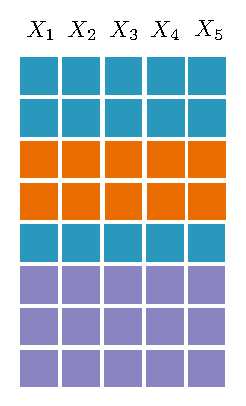
\includegraphics[width=0.5791\linewidth]{figures/grid-1}
      %\end{center}
    \end{minipage} \hspace{10pt}\begin{minipage}[t]{0.3\linewidth}
      %\begin{center}
        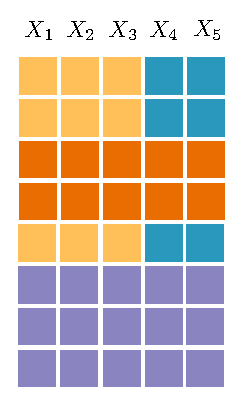
\includegraphics[width=0.5832\linewidth]{figures/grid-2}
      %\end{center}
    \end{minipage}
    \hspace{10pt}\begin{minipage}[t]{0.3\linewidth}
      %\begin{center}
        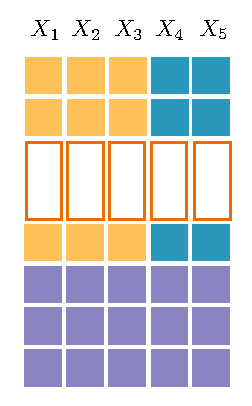
\includegraphics[width=0.59535\linewidth]{figures/grid-3}
      %\end{center}
    \end{minipage}
  \vspace{5pt}
  \raisebox{0pt}{\begin{minipage}[t]{0.3\linewidth}
        %\begin{center}
          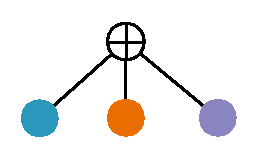
\includegraphics[width=0.5791\linewidth]{figures/learnspn-1}
        %\end{center}
      \end{minipage}}\hspace{4pt}\raisebox{-20pt}{\begin{minipage}[t]{0.3\linewidth}
        %\begin{center}
          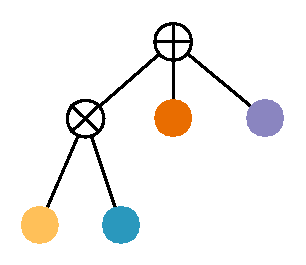
\includegraphics[width=0.6723\linewidth]{figures/learnspn-2}
        %\end{center}
      \end{minipage}}\hspace{1pt}\raisebox{-18pt}{\begin{minipage}[t]{0.3\linewidth}
        %\begin{center}
          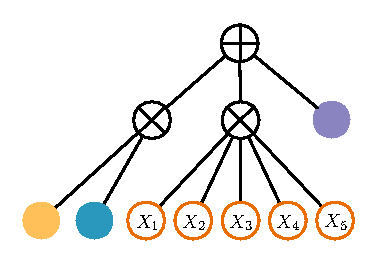
\includegraphics[width=0.81\linewidth]{figures/learnspn-3}
        %\end{center}
      \end{minipage}}\par\bigskip
  remember SPNs are built via \emph{hierarchical co-clustering}, learning
  features as \textbf{\emph{recursive data
      crawlers}}!\customcitenomark{Vergari2015}\customcitenomark{Gens2013}
\end{frame}



\begin{frame}[t]
  \frametitle{\highlighttext[bgrey2]{Automating density estimation}}
  \footnotesize
  
  \begin{enumerate}
    \setlength{\itemindent}{0pt}
  %\setlength{\leftmargini}{-5pt}  
    %\setlength{\leftmargin}{-5pt}
    % \setlength{\parskip}{-3pt}
  \item decide a \textbf{parametric form} for the estimator
    \begin{itemize}
      \setlength{\itemindent}{-10pt}
      \scriptsize
    \item  a parametric form for individual RVs 
\item the dependency structure parametric form
  \hfill$\color{violet}\boldsymbol\Rightarrow$
  {\scriptsize\highlighttext[tomato0]{\emph{\textbf{SPN structure}}}} 
    \end{itemize}
  \item \textbf{fit the estimator} to the data  \hfill$\color{violet}\boldsymbol\Rightarrow$
  {\scriptsize\highlighttext[tomato4]{\emph{\textbf{LearnSPN}}}} 
    \begin{itemize}
      \setlength{\itemindent}{-10pt}
      \scriptsize
    \item fit model structure
      \item fit model parameters
    \end{itemize}
  \item perform \textbf{inference \emph{ad libitum}}
    \begin{itemize}\scriptsize
      \setlength{\itemindent}{-10pt}
    \item several kinds of probabilistic queries \hfill$\color{violet}\boldsymbol\Rightarrow$
  {\scriptsize\highlighttext[tomato4]{\emph{\textbf{EVI, MAR, CON,\dots}}}} 
    \item compute statistics, metrics, descriptors
      \item make sense of the data and the model (\textbf{interpretability})\hfill$\color{violet}\boldsymbol\Rightarrow$
  {\scriptsize\highlighttext[tomato4]{\emph{\textbf{visualizing
          filters}}}} 
      \item\dots
    \end{itemize}
  

    \item \textbf{(\emph{re-})use knowledge} in other tasks \hfill$\color{violet}\boldsymbol\Rightarrow$
  {\scriptsize\highlighttext[tomato4]{\emph{\textbf{SPAE embeddings
          and routines}}}} 
  \end{enumerate}
\end{frame}


\begin{frame}[t]
  \frametitle{\highlighttext[peas1]{Mixed Sum-Product Networks (MSPNs)}% \footnote{Ex
      % Manichean Sum-Product Networks}
  }
  \footnotesize

  Relieving practitioners from imposing parametric forms for RVs and
  their interactions\par
  \begin{minipage}{1.0\linewidth}
  % \vspace{2pt}
      \raggedleft
      $\color{violet}\boldsymbol\Rightarrow$
      \scriptsize
 \emph{general strong assumptions---e.g., gaussianity---may not hold
   in practice}
\end{minipage}\par
\begin{minipage}{1.0\linewidth}
  \vspace{2pt}
      \raggedleft
      $\color{violet}\boldsymbol\Rightarrow$
      \scriptsize
 \emph{specific knowledge  over hybrid domains is often beyond users' possibilities}
\end{minipage}\par\bigskip

  LearnSPN and its variants are tailored towards specific parametric
  assumptions---gaussian~\customcite{Jaini2016}, multinomial~\customcite{Gens2013} or poisson data~\customcite{Molina2017a}\par\bigskip

  \textbf{\emph{Mixed Sum-Product Networks}} (\textbf{MSPNs}) combine
  SPNs with {\textbf{piecewise polynomial approximations}} to provide a
  density estimator \textbf{without making parametric form assumptions} when 
  \begin{itemize}
    \setlength{\itemsep}{-3pt}
  \item seeking \highlighttext[bgrey0]{\emph{\textbf{RV dependencies}}} (column splits)
    \item determining \highlighttext[bgrey1]{\emph{\textbf{instance clustering}}} (row splits)
    \item modeling \highlighttext[bgrey2]{\textbf{\emph{univariate distributions}}} (leaf growing)
  \end{itemize}

\end{frame}

\begin{frame}[t]
  \frametitle{\highlighttext[peas2]{LearnMSPN: decomposing RVs I}}
  \footnotesize

  Looking for RV dependency through an empirical estimator for
  R{\'e}nyi's Maximum Correlation Coefficient~\parencite{Renyi1959},
  the \emph{\textbf{Randomized Dependency Coefficient}} (\textbf{RDC})~\parencite{LopezPaz2013}.\par\bigskip


  RVs $X_{i}$ and $X_{j}$ are independent iff for two
  samples $\mathcal{D}_{X_{i}}=\{x^{m}_{i}|x^{m}_{i}\sim X_{i}\}_{m=1}^{M}$
  and $\mathcal{D}_{X_{j}}=\{x^{m}_{j}|x^{m}_{j}\sim X_{j}\}_{m=1}^{M}$
  $\mathsf{RDC}(\mathcal{D}_{X_{i}}, \mathcal{D}_{X_{j}})\approx 0$.\par\bigskip

  I. Preserve marginal structure by going through the \highlighttext[olive5]{\emph{\textbf{empirical cdf}}}:
  
 \begin{equation*}
  \mathcal{C}_{X_{i}}=\bigg\{ {\color{olive5}\frac{1}{M}\sum\nolimits_{r=1}^{M}\mathds{1}\{v_{i}^r \leq v_{i}^{m}\}}\bigg|v^{m}_{i}\in\mathcal{D}_{X_{i}}\bigg\}_{m=1}^{M}
  \label{eq:copula}
\end{equation*}

II. Randomly project to a
\highlighttext[pink2]{\textbf{\emph{$k$-dimensional gaussian space}}},
and then apply a \highlighttext[brown3]{\emph{\textbf{non-linearity}}} $\sigma$.
%

\begin{equation*}
  \phi(\mathcal{C}_{X_{i}})={\color{brown3}\sigma}({\color{pink2}\mathbf{w}}\cdot\mathcal{C}_{X_{i}}^{T}+{\color{pink2}b}), ({\color{pink2}\mathbf{w}}, {\color{pink2}b})\sim\mathcal{N}(\mathbf{0}_{k}, s\mathbf{I}_{k\times k})
  \label{eq:nonlinear}
\end{equation*}

\customcitenomark{Molina2017b}
\end{frame}

\begin{frame}[t]
  \frametitle{\highlighttext[peas2]{LearnMSPN: decomposing RVs II}}
  \footnotesize

  III. The RDC is the largest canonical correlation analysis (CCA) coefficient
  \begin{equation*}
  \mathsf{RDC}(\mathcal{D}_{X_{i}}, \mathcal{D}_{X_{j}}) =\sup\nolimits_{{\color{pink3}\boldsymbol\beta}, {\color{olive5}\boldsymbol\gamma}}\rho({\color{pink3}\boldsymbol\beta}^{T}\phi(\mathcal{C}_{X_{i}}),{\color{olive5}\boldsymbol\gamma}^{T}\phi(\mathcal{C}_{X_{j}})).
\end{equation*}

where  $\rho^{2}$  is the solution of the eigenproblem for the CCA over $\phi(\mathcal{C}_{X_{i}})$ and $\phi(\mathcal{C}_{X_{j}})$:
\begin{equation*}
  \begin{pmatrix}
0 & \Sigma^{-1}_{ii}\Sigma_{ij} \\ 
\Sigma^{-1}_{jj}\Sigma_{ji} & 0
\end{pmatrix}
\begin{pmatrix}
{\color{pink3}\boldsymbol\beta} \\ 
{\color{olive5}\boldsymbol\gamma}
\end{pmatrix}=\rho^2
\begin{pmatrix}
{\color{pink3}\boldsymbol\beta} \\ 
{\color{olive5}\boldsymbol\gamma}
\end{pmatrix},
\label{eq:cancor}
\end{equation*}
where the covariance block matrices involved are: 
$$\Sigma_{ij}=\text{cov}(\phi(\mathcal{C}_{X_{i}}),\phi(\mathcal{C}_{X_{j}})), \Sigma_{ji}=\text{cov}(\phi(\mathcal{C}_{X_{j}}),\phi(\mathcal{C}_{X_{i}})),$$
$$\Sigma_{ii}=\text{cov}(\phi(\mathcal{C}_{X_{i}}),\phi(\mathcal{C}_{X_{i}})), \Sigma_{jj}=\text{cov}(\phi(\mathcal{C}_{X_{j}}),\phi(\mathcal{C}_{X_{j}})).$$

% In the end, the actual value for the RDC coefficient is the largest canonical correlation coefficient:

\customcitenomark{Molina2017b}

\end{frame}



\begin{frame}[t]
  \frametitle{\highlighttext[peas2]{LearnMSPN: clustering}}
  \footnotesize

  Clustering hybrid data highly depends on the metric space
  employed:\par
  \begin{minipage}{1.0\linewidth}
  % \vspace{2pt}
      \raggedleft
      $\color{violet}\boldsymbol\Rightarrow$
      \scriptsize
 \emph{e.g. K-Means relies on gaussianity}
\end{minipage}\par\bigskip

  
  We employ the RDC pipeline to project into a homogeneous space
  in which clusters may be more easily separable.\par
  Given a samples $\mathcal{D}_{\mathbf{X}}$ over RVs $\mathbf{X}$ we:
  \begin{enumerate}
  \item compute
    ${\mathcal{E}}=\{{\color{olive5}\mathcal{C}}(\mathcal{D}_{X_{i}})|\mathcal{D}_{X_{i}}\}_{i=1}^{n}.$
    via the \highlighttext[olive5]{\textbf{\emph{empirical copula
          transform}}}
\item then project all features into  a new
  \highlighttext[pink2]{\emph{\textbf{$k$-dimensional}}}
  \highlighttext[brown3]{\emph{\textbf{non-linear}}} space
  \item finally, we apply clustering---e.g. safely K-Means---to obtain
    $c$ clusters\par
    \begin{minipage}{1.0\linewidth}
  % \vspace{2pt}
      \raggedleft
      $\color{violet}\boldsymbol\Rightarrow$
      \scriptsize
 \emph{$c=2$ for deeper SPNs~\parencite{Vergari2015}}
\end{minipage}
  \end{enumerate}\par\bigskip

Comparable to employing the \emph{\textbf{Gower distance}}---if one can make parametric assumptions\customcitenomark{Molina2017b}
\end{frame}


\begin{frame}[t]
  \frametitle{\highlighttext[peas3]{LearnMSPN: leaf distribution modeling}}
  \footnotesize

  Approximate univariate leaf probability mass or density functions with
  \textbf{\emph{piecewise polynomials}}\par
  \begin{minipage}{1.0\linewidth}
  \vspace{-15pt}
      \raggedleft
      $\color{violet}\boldsymbol\Rightarrow$
      \scriptsize
 \emph{unwrapping the
  whole MSPN polynomial for symbolic evaluation}
\end{minipage}

  \begin{figure}[t] 
\centering
 %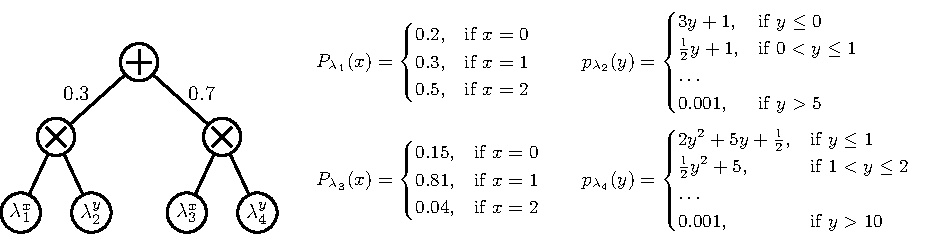
\includegraphics[width=0.5\columnwidth]{figures/mspn}\quad
 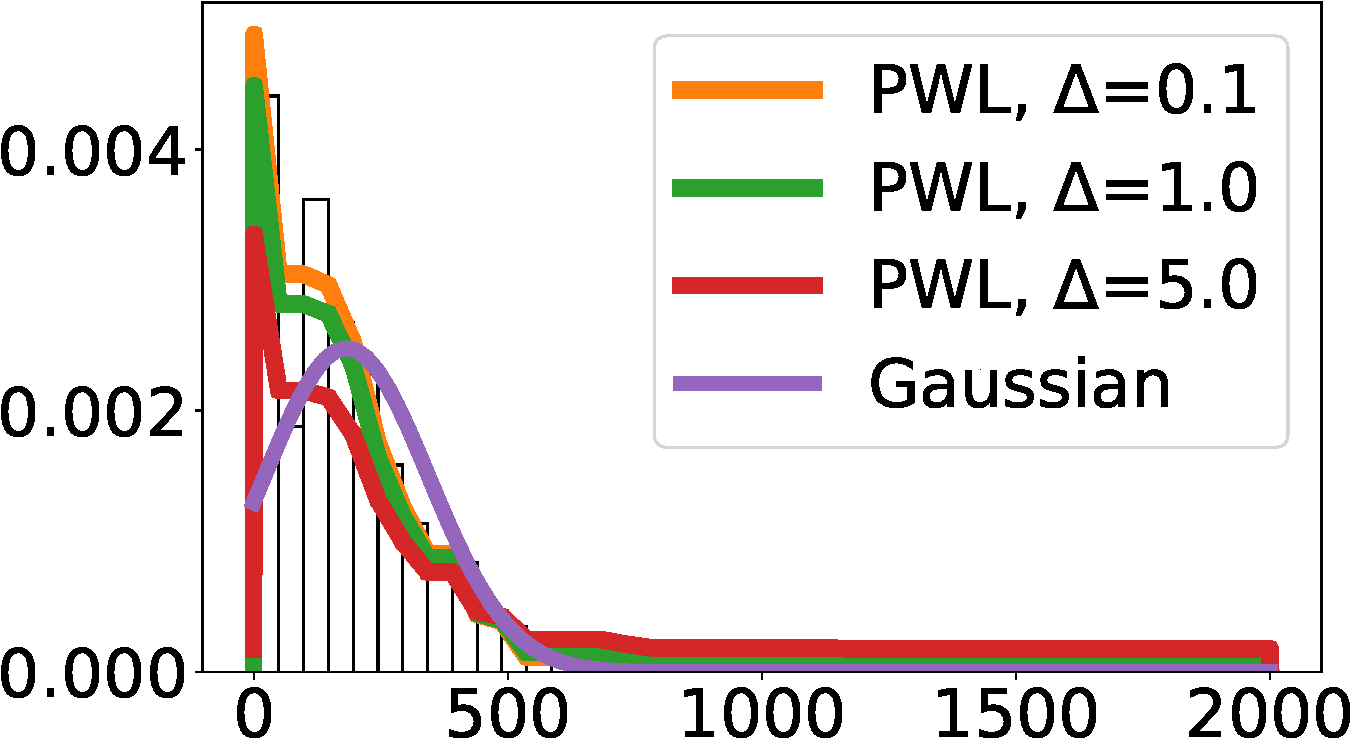
\includegraphics[width=0.34\columnwidth]{figures/australian-12-crop}\hspace{25pt}
  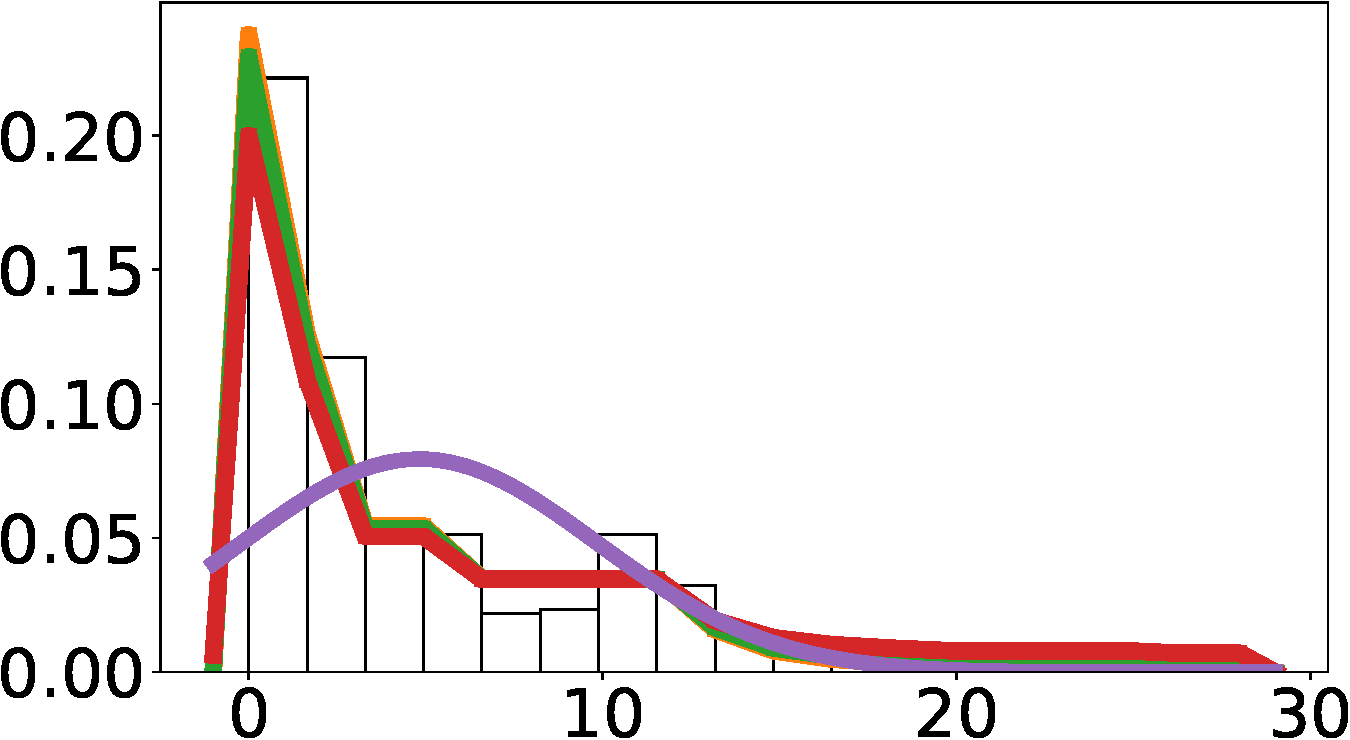
\includegraphics[width=0.34\columnwidth]{figures/australian-2-crop}

\end{figure}

  \highlighttext[bgrey1]{\emph{\textbf{Degree 0 approximations}}}:
  piecewise constants, i.e. {\emph{\textbf{histograms}}}\par
  \begin{minipage}{1.0\linewidth}
  \vspace{5pt}
      \raggedleft
      $\color{violet}\boldsymbol\Rightarrow$
      \scriptsize
 % \emph{unwrapping the
 % whole MSPN polynomial for symbolic evaluation}
      adaptive bins by fitting an irregular
  histogram by optimizing a penalized
  log-likelihood~\parencite{Rozenholc2010}% and Laplacian smoothing $\Delta$
\end{minipage}%\par\bigskip

  

\highlighttext[bgrey2]{\emph{\textbf{Degree 1 approximations}}}:
piecewise linear\par
\begin{minipage}{1.0\linewidth}
  \vspace{5pt}
      \raggedleft
      $\color{violet}\boldsymbol\Rightarrow$
      \scriptsize
reframing it into a supervised task,
  fitting a piecewise linear model\par via \emph{\textbf{unimodal isotonic regression}}~\parencite{Frisen1986}
\end{minipage}
\customcitenomark{Molina2017b}
\end{frame}


\begin{frame}[t]
  \frametitle{\highlighttext[peas4]{MSPNs: inference over hybrid domains}}
  \footnotesize

      Toy \emph{\textbf{symbol grounding}} with MSPN: embed MNIST digits into a $16$-d
    continuous space $\mathbf{X}$ and augment them with binary codes $\mathbf{Y}$
    for semantic features:\par
\hspace{20pt}\begin{minipage}{0.9\linewidth}
  \vspace{2pt}
      \raggedright
(i) a vertical stroke,
(ii) a circle,
(iii) a left curvy stroke,\par
(iv) a right curvy stroke,
(v) a horizontal stroke,
(vi) a double curve stroke
\end{minipage}
\begin{minipage}{1.0\linewidth}
  \vspace{5pt}
      \raggedleft
      $\color{violet}\boldsymbol\Rightarrow$
      \scriptsize
 \emph{the code for 3 is therefore: $\mathbf{y}_{3}=(0,0,1,0,1,1)$}
\end{minipage}


  \begin{figure}[t]
  
    \begin{minipage}{0.2\linewidth}
\vspace{-13pt}
    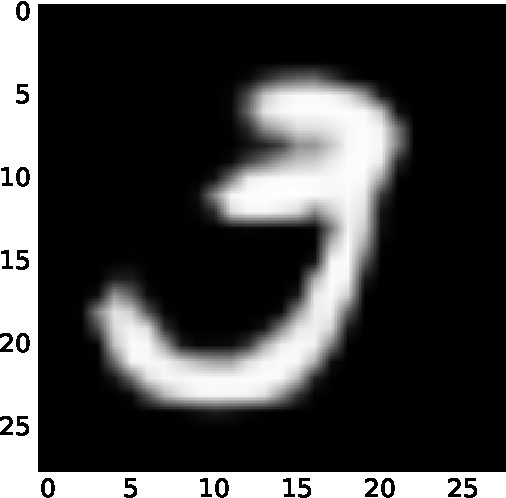
\includegraphics[width=0.47\linewidth]{figures/mpe-12}\\
    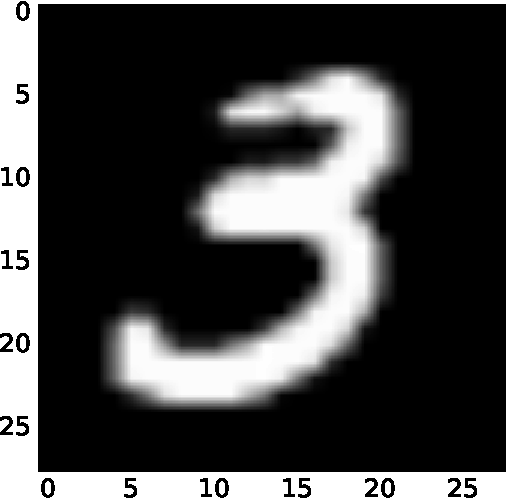
\includegraphics[width=0.47\linewidth]{figures/nn-sample-12}
\end{minipage}\hspace{-30pt}\begin{minipage}{0.18\linewidth}
    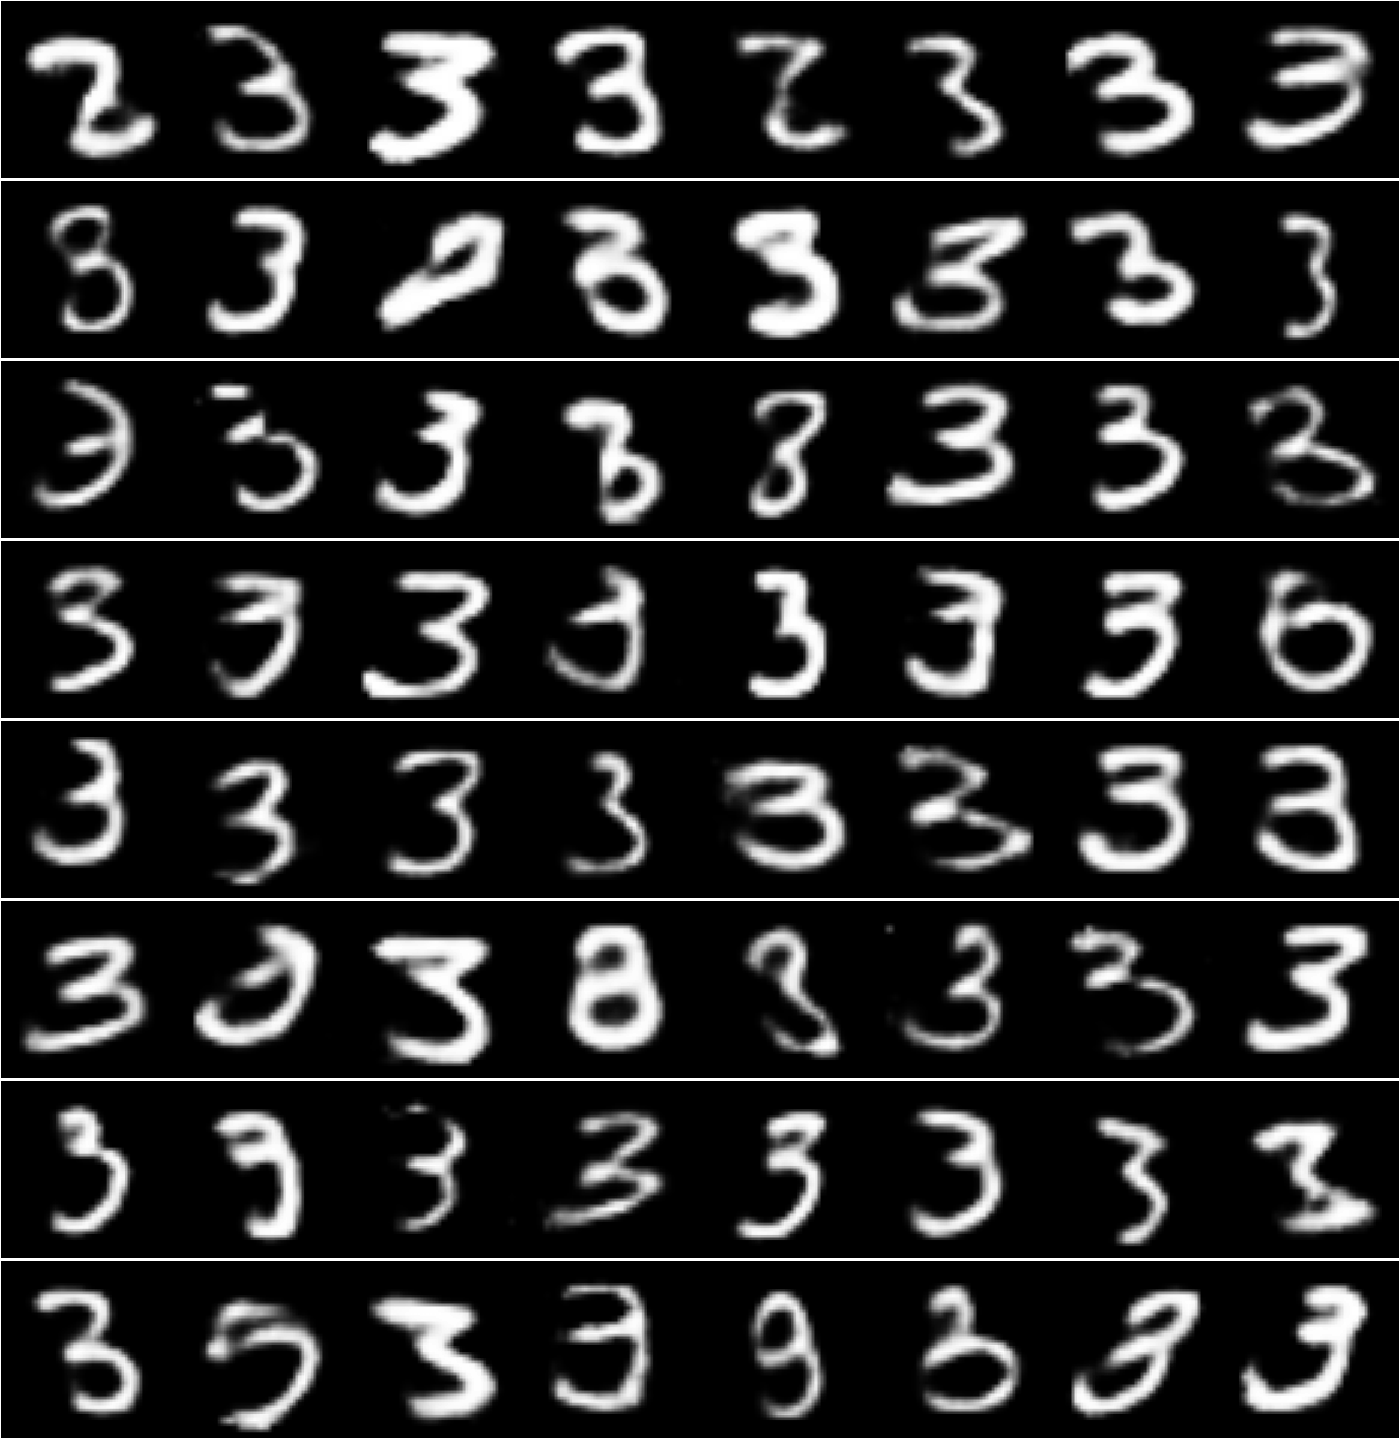
\includegraphics[width=1.0\columnwidth]{figures/cond-samples-12}\\
    %$\{0,0,1,0,1,1\}$
    \highlighttext[olive4]{\scriptsize\textbf{\emph{(0,0,1,0,1,1)}}}
\end{minipage}\hspace{5pt}\begin{minipage}{0.2\linewidth}
\vspace{-13pt}
    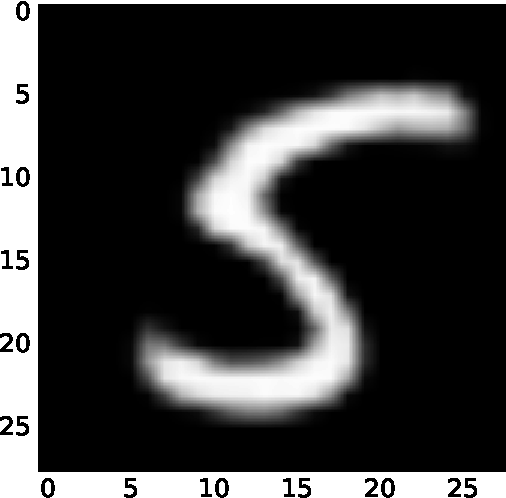
\includegraphics[width=0.47\linewidth]{figures/mpe-15}\\
    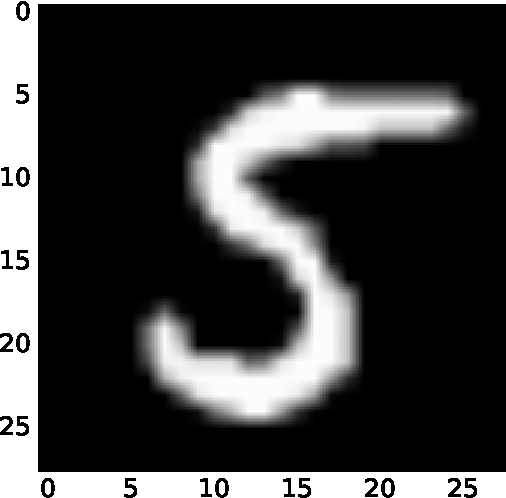
\includegraphics[width=0.47\linewidth]{figures/nn-sample-15}
\end{minipage}\hspace{-30pt}\begin{minipage}{0.18\linewidth}
    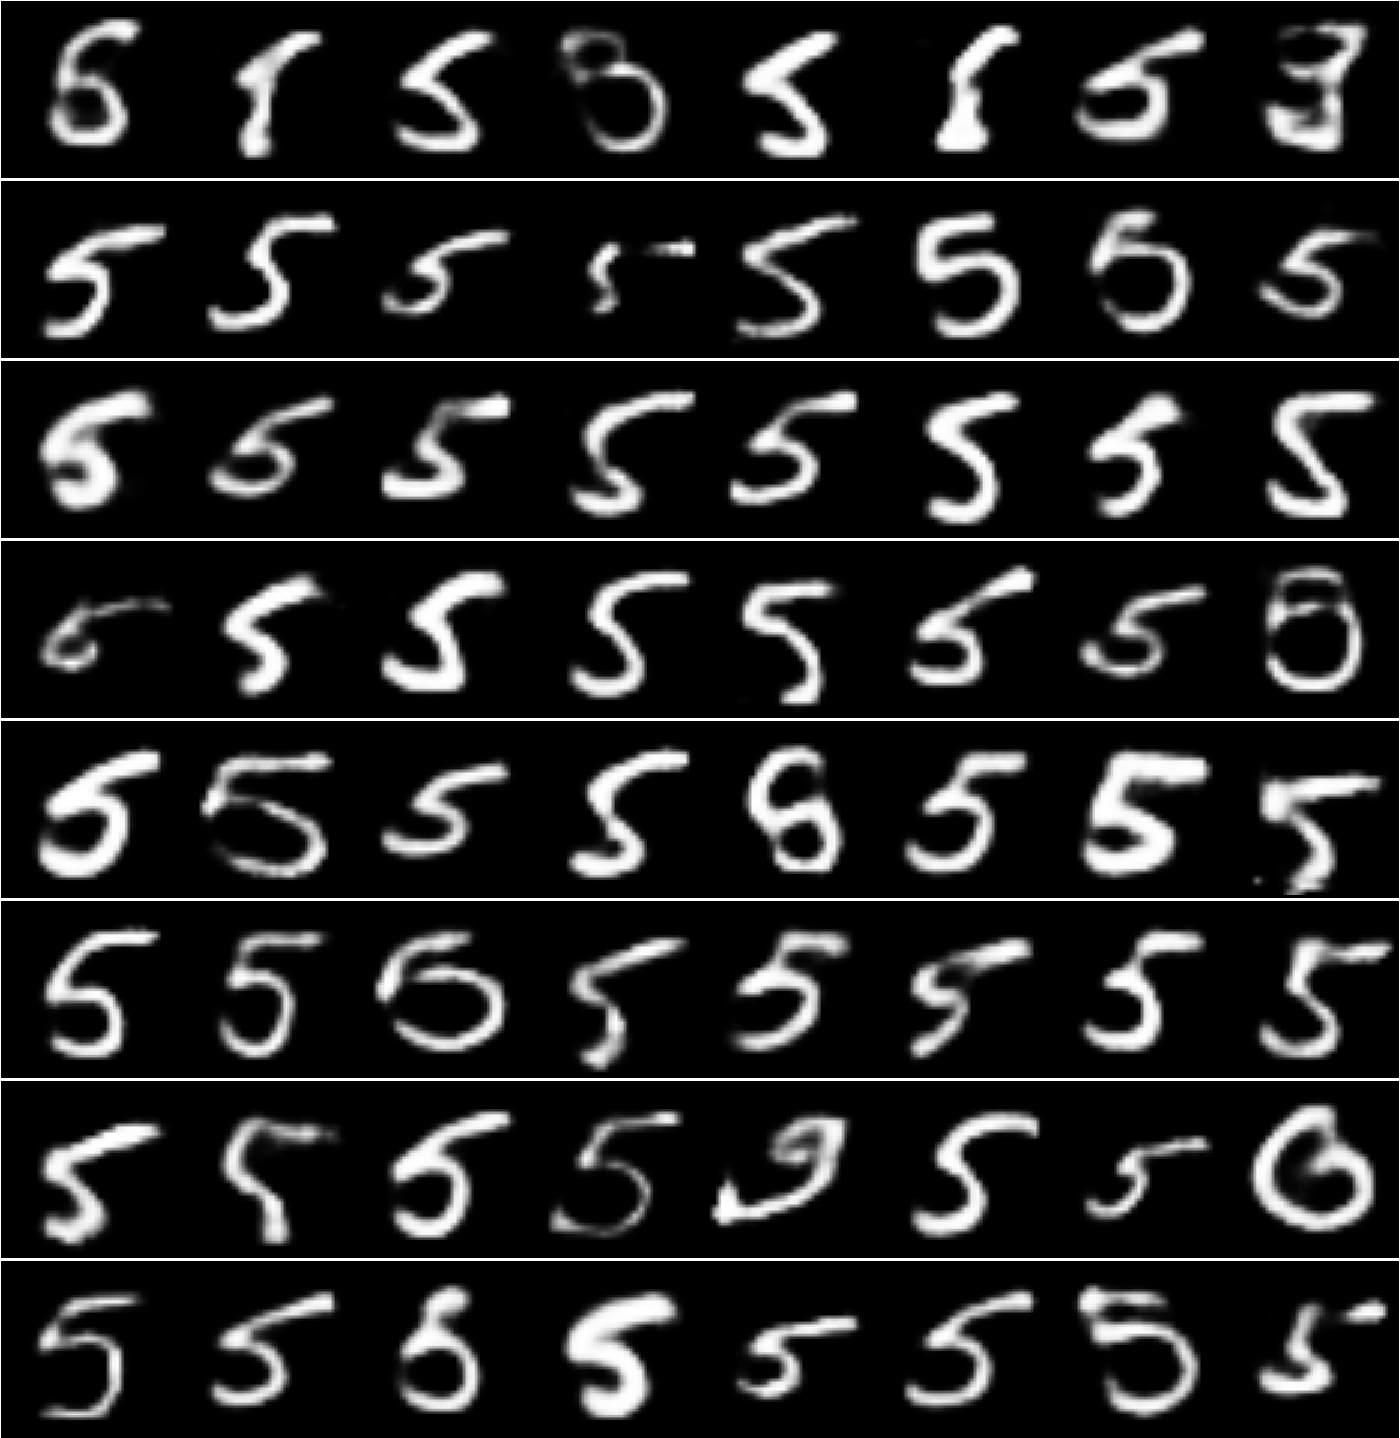
\includegraphics[width=1.0\columnwidth]{figures/cond-samples-15}\\
    % $\{0,0,1,1,1,0\}$
    % \highlighttext[blue]{\textbf{\emph{b}}}
    \highlighttext[olive4]{\scriptsize\textbf{\emph{(0,0,1,1,1,0)}}}
\end{minipage}\hspace{5pt}\begin{minipage}{0.18\linewidth}
    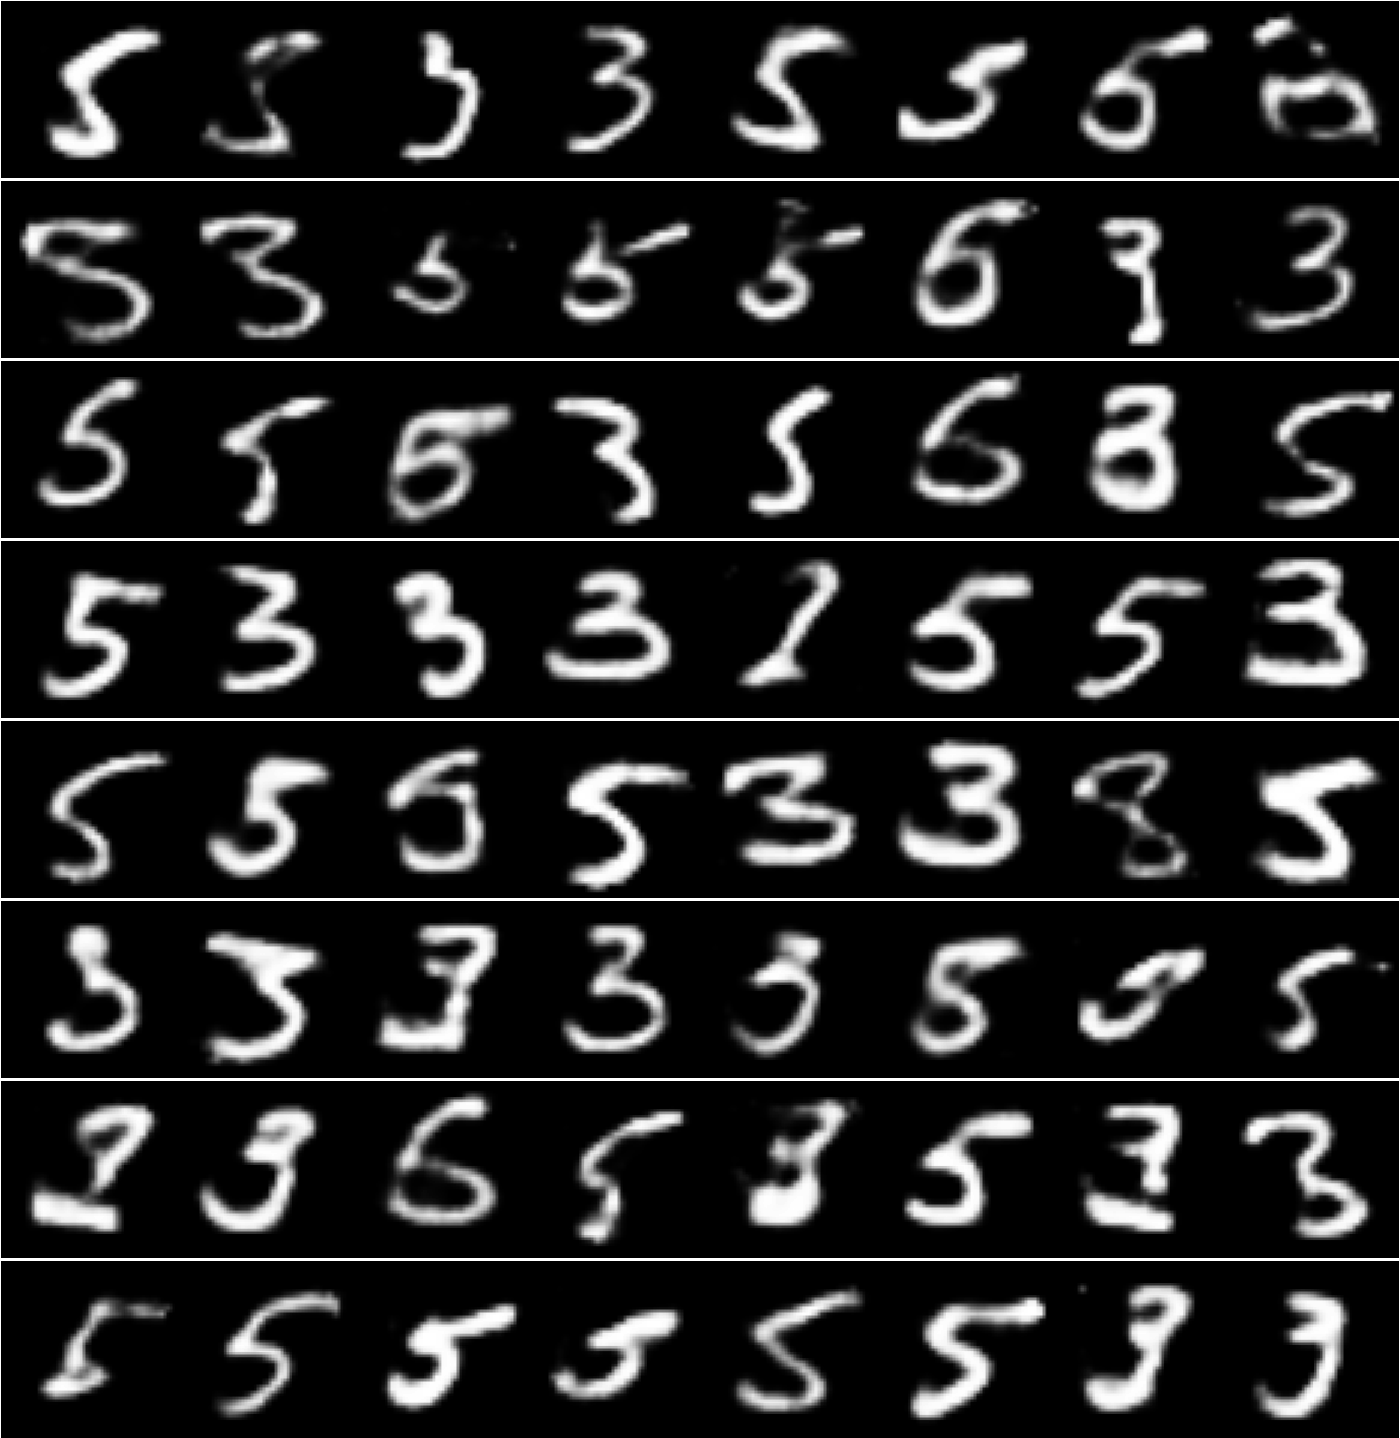
\includegraphics[width=1.0\columnwidth]{figures/cond-samples-16}\\
    %$\{0,0,1,1,1,1\}$
    %\centering\highlighttext[orange]{\textbf{\emph{c}}}
    \hspace{10pt}\highlighttext[brown4]{\scriptsize\textbf{\emph{(0,0,1,1,1,1)}}}
\end{minipage}\hspace{5pt}\begin{minipage}{0.18\linewidth}
    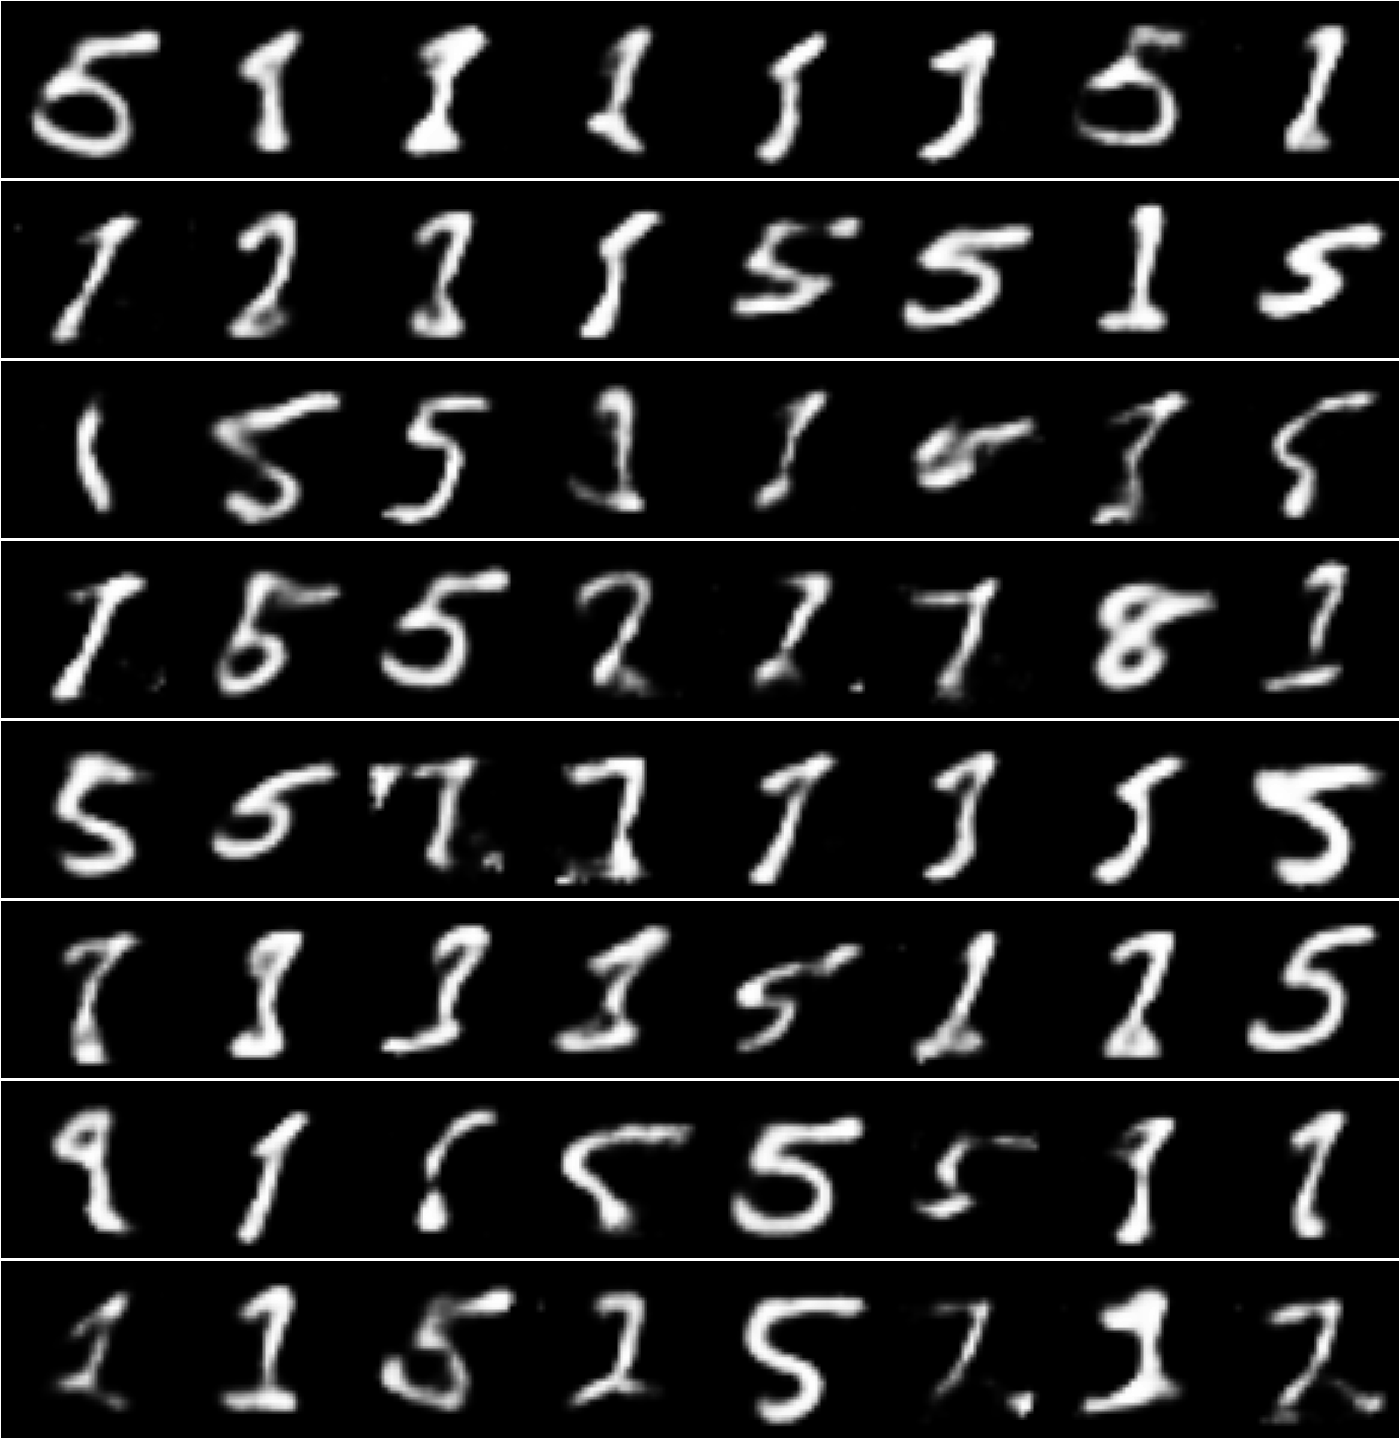
\includegraphics[width=1.0\columnwidth]{figures/cond-samples-47}\\
    % \begin{center}$\{1,0,1,1,1,0\}$\end{center}
    %\centering\highlighttext[orange]{\textbf{\emph{d}}}
    \hspace{10pt}\highlighttext[brown4]{\scriptsize\textbf{\emph{(1,0,1,1,1,0)}}}
\end{minipage}

\customcitenomark{Molina2017b}
\end{figure}

Model $p(\mathbf{X}, \mathbf{Y}_{c}, c)$ with an MSPN and perform:
Easily perform {\textbf{\emph{MPE and conditional sampling}}} from $p(\mathbf{X}|\mathbf{y}_{c})$
over \highlighttext[olive4]{\textbf{existing class codes}} $\mathbf{y}_c$ and \highlighttext[brown4]{\textbf{invented ones}}.


\end{frame}


\begin{frame}[t]
  \footnotesize
  \frametitle{\highlighttext[peas5]{MSPNs: privileged information learning}}

  Efficient marginalization in MSPNs allows to leverage additional
   RVs at training time as \textbf{\emph{privileged information}}
  \begin{figure}
    \centering
    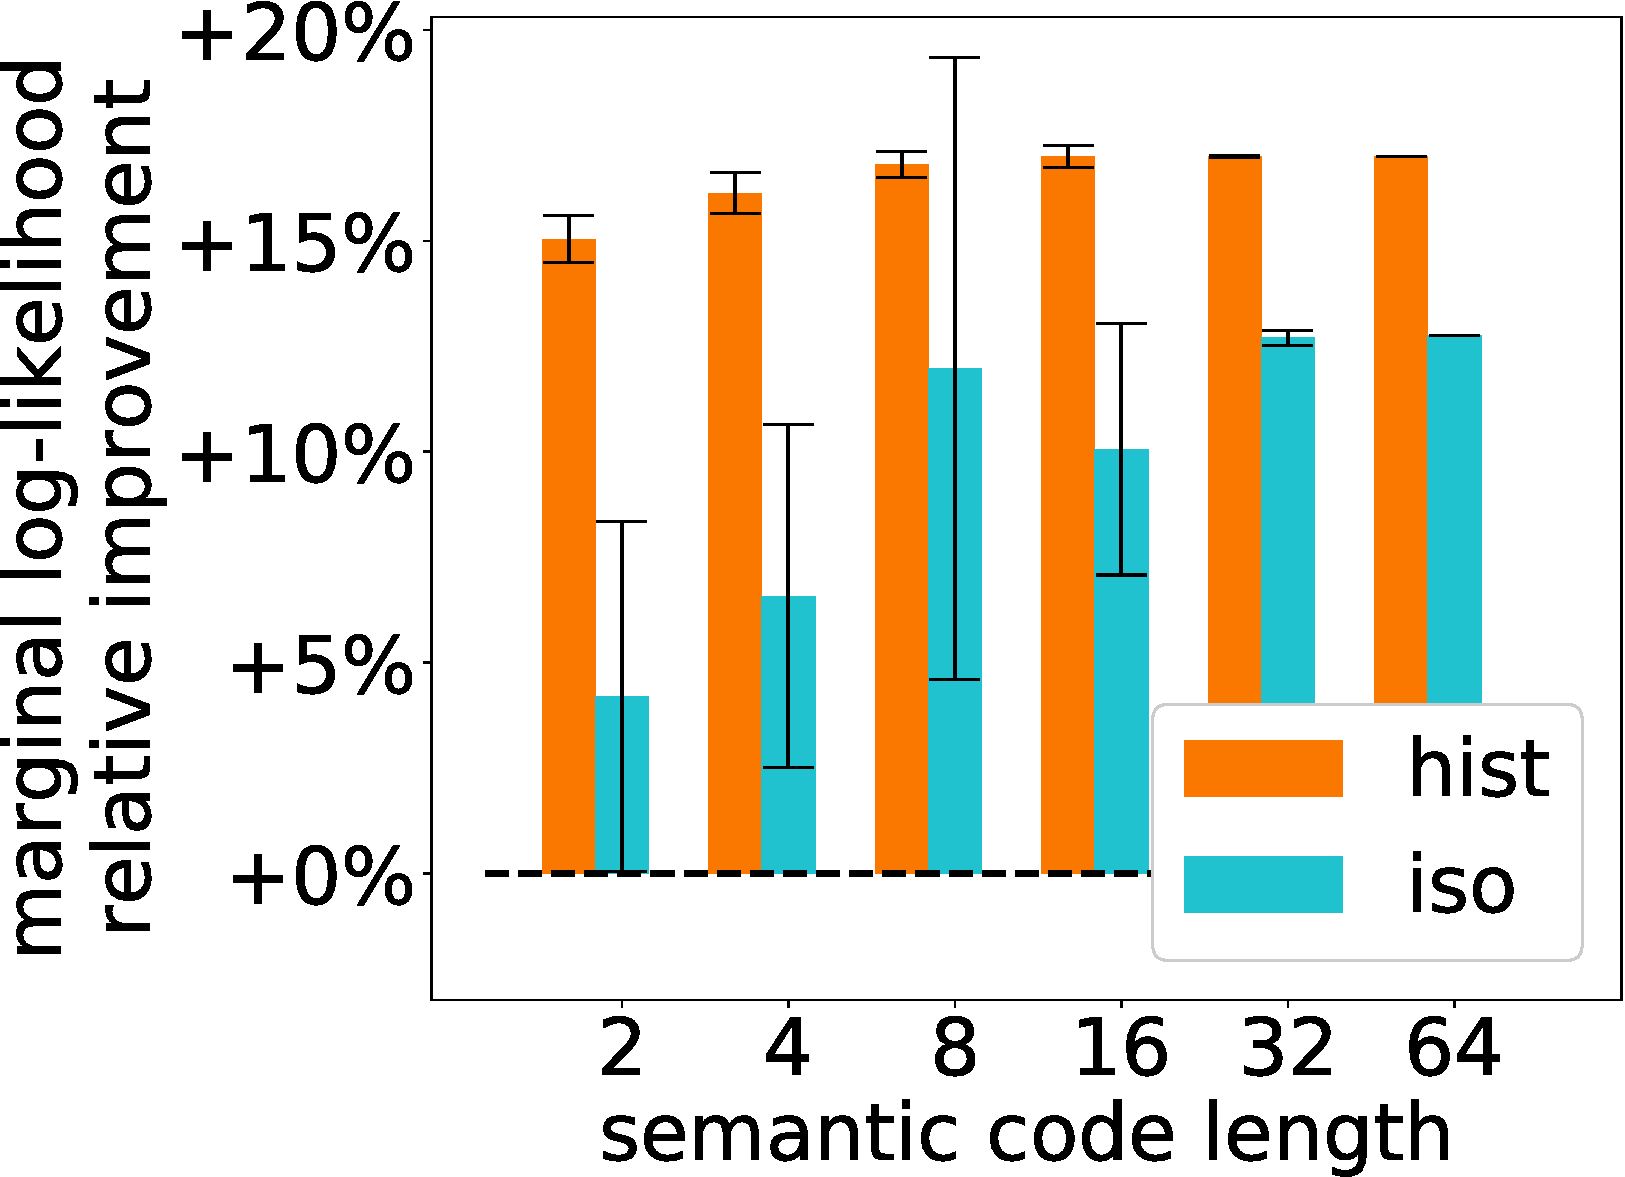
\includegraphics[width=0.38\columnwidth]{figures/marg-test-ll-crop}\hspace{20pt}
    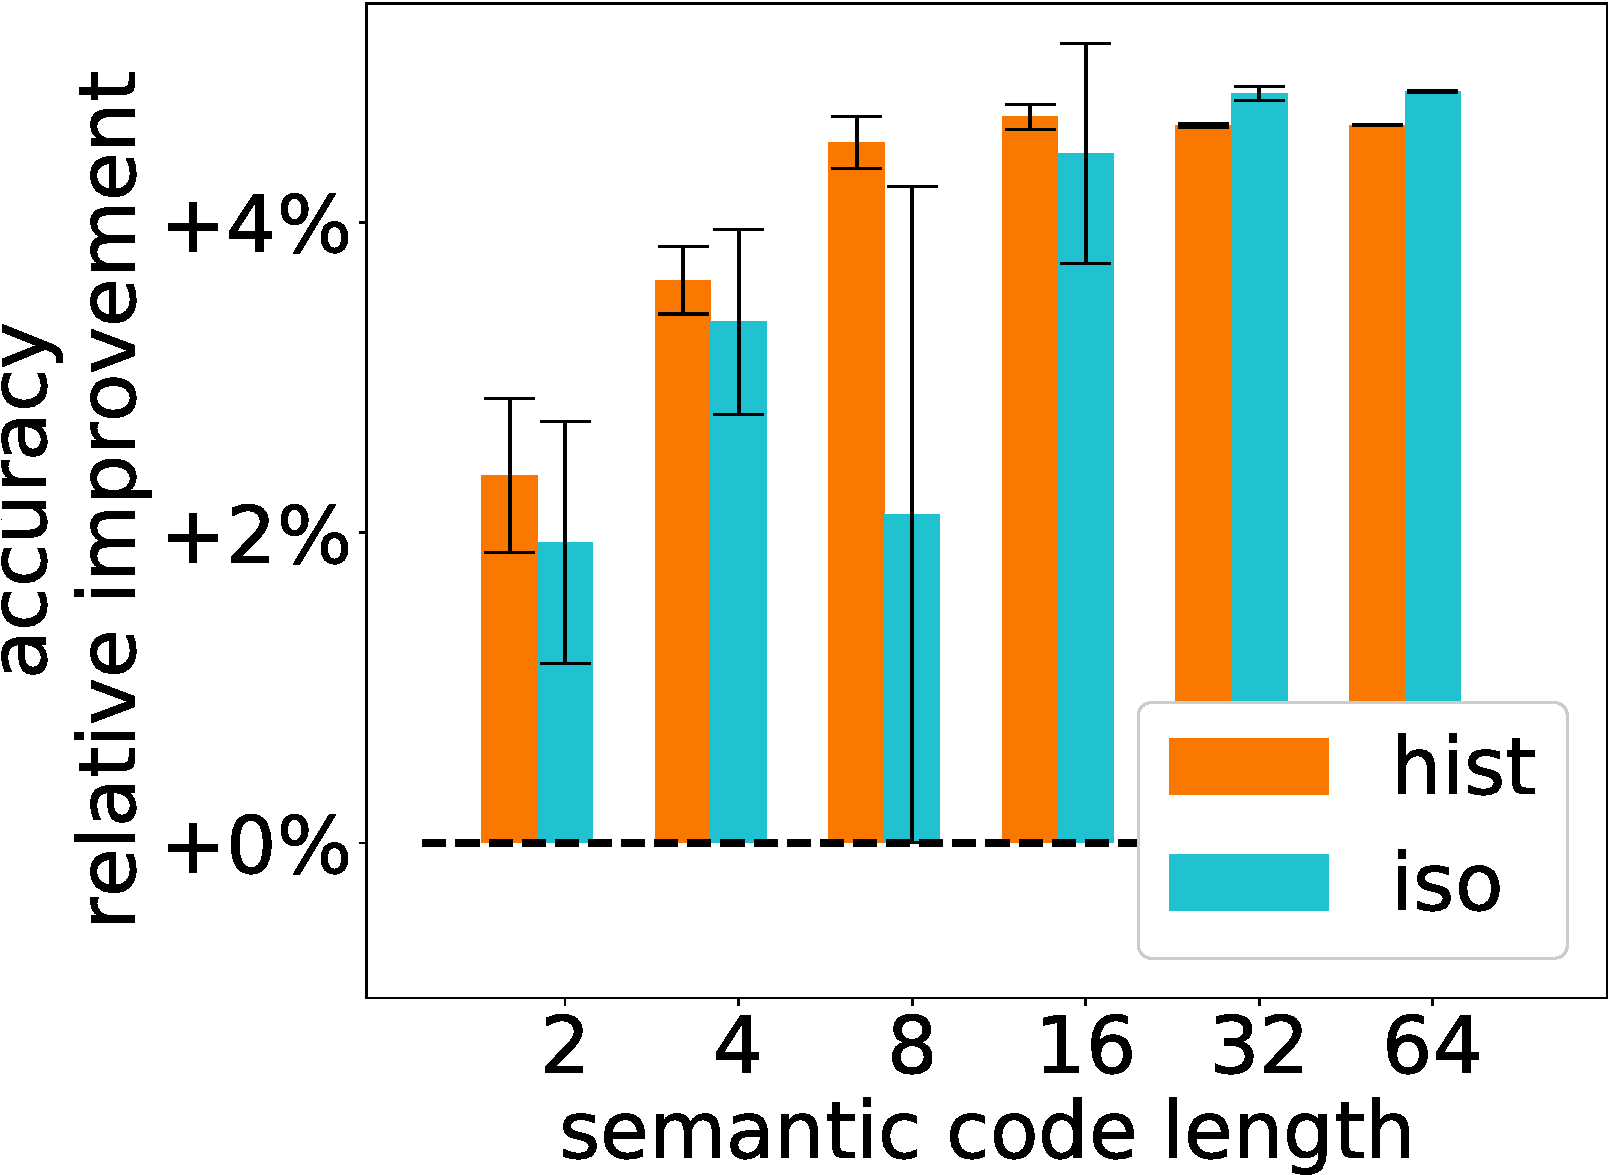
\includegraphics[width=0.38\columnwidth]{figures/test-mpe-acc-crop}\\
    \hspace{30pt}\highlighttext[pink4]{\emph{\textbf{a}}}\hspace{120pt} \highlighttext[olive4]{\emph{\textbf{b}}}
  \end{figure}

  Randomly increasing the semantic codes $\mathbf{Y}_{c}$ helps
  modeling both the \highlighttext[pink4]{\emph{\textbf{marginal
        likelihood}}} $p(\mathbf{X})$ and the \highlighttext[olive4]{\emph{\textbf{predictive accuracy}}} on
  the class $c$ at test time

  \begin{minipage}{1.0\linewidth}
  \vspace{5pt}
      \raggedleft
      $\color{violet}\boldsymbol\Rightarrow$
      \scriptsize
 \emph{towards stacking density estimators}
\end{minipage}

  \customcitenomark{Molina2017b}

\end{frame}


\begin{frame}[t]
  \frametitle{\highlighttext[peas5]{MSPNs: orchestrating inference}}
  \footnotesize

  
  Split RVs into two halves---$\mathbf{X}_{l}$, $\mathbf{X}_{r}$,
  $\mathbf{X}_{u}$,  and
  $\mathbf{X}_{d}$---and learn one autoencoder $f$ on each RV set
  \emph{independently}.
  They act as different domains.\par\bigskip
  Learn one MSPN $M_{ud}$ to model $P(f_{u}(\mathbf{X}_{u}),
  f_{d}(\mathbf{X}_{d}))$ (resp. $M_{lr}$ and $P(f_{l}(\mathbf{X}_{l}), f_{r}(\mathbf{X}_{r}))$).

  Given one half test image, \highlighttext[darkred]{\textbf{predict}}
  the other half.
  \begin{minipage}{1.0\linewidth}
  \vspace{5pt}
      \raggedleft
      $\color{violet}\boldsymbol\Rightarrow$
      \scriptsize
 \emph{$M_{ud}$ fills and glues the embedding spaces of $f_{u}$ and $f_{d}$}
\end{minipage}
  \begin{figure}[t]
\begin{minipage}{0.6\linewidth}
\vspace{0pt}
    \setlength{\tabcolsep}{-0.1pt}
    \begin{tabular}{rrrrrrrrr}
    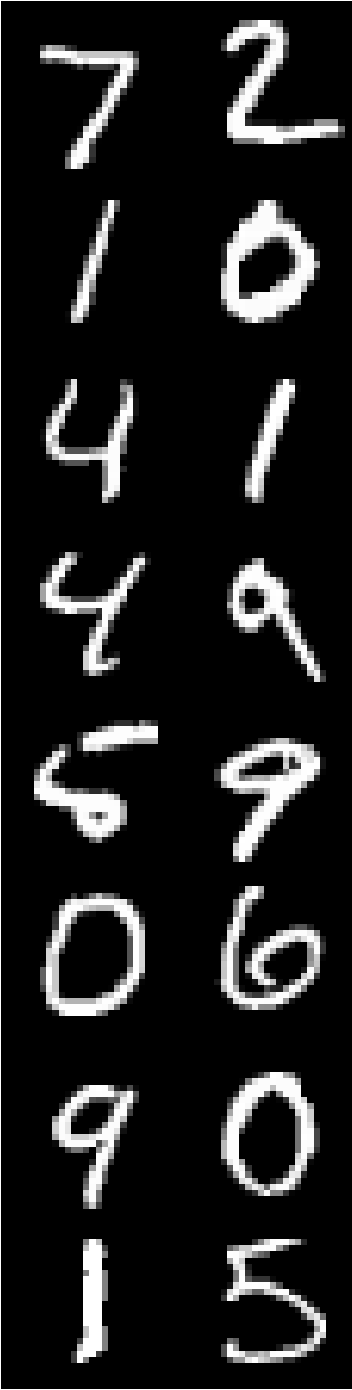
\includegraphics[width=0.14\columnwidth]{figures/orig-16-crop}&$\quad\quad$&
    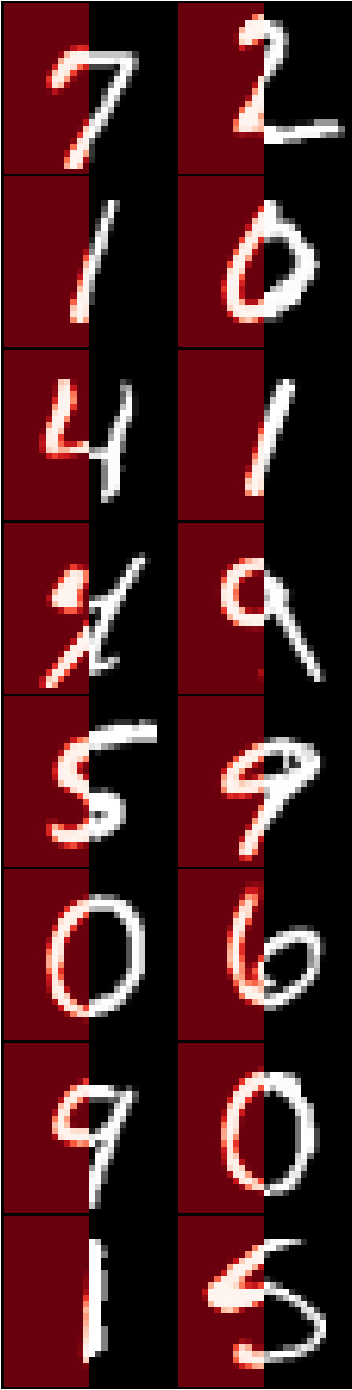
\includegraphics[width=0.14\columnwidth]{figures/dec-left-16-crop}&$\quad\quad$&
    \includegraphics[width=0.14\columnwidth]{figures/dec-right-16-crop}&$\quad\quad$&
    \includegraphics[width=0.14\columnwidth]{figures/dec-up-16-crop}&$\quad\quad$&
    \includegraphics[width=0.14\columnwidth]{figures/dec-down-16-crop}
    \end{tabular}
  \end{minipage}

  
\end{figure}
\customcitenomark{Molina2017b}
\end{frame}


\begin{frame}[t]
  \footnotesize
  \frametitle{\highlighttext[peas5]{MSPNs: hybrid measures computation}}

  Recall, an MSPN encodes a polynomial over leaf piecewise
  polynomials.\par
  \begin{minipage}{1.0\linewidth}
  \vspace{5pt}
      \raggedleft
      $\color{violet}\boldsymbol\Rightarrow$
      \scriptsize
 \emph{managing complexity by divide-et-impera representations!}
\end{minipage}\par\bigskip
  

   Employing a symbolic solver to evaluate the overall network
   polynomial to easily compute information-theoretic measures for
   hybrid domains,\par e.g. \highlighttext[bgrey2]{\emph{\textbf{hybrid mutual information}}}
   
  \begin{figure}[t]
    \centering
    \includegraphics[width=0.4\columnwidth]{figures/MI_graph}
  \end{figure}

  \customcitenomark{Molina2017b}
\end{frame}

\begin{frame}[t]
  \frametitle{\highlighttext[bgrey2]{Automating density estimation}}
  \footnotesize
  
  \begin{enumerate}
    \setlength{\itemindent}{0pt}
  %\setlength{\leftmargini}{-5pt}  
    %\setlength{\leftmargin}{-5pt}
    % \setlength{\parskip}{-3pt}
  \item decide a \textbf{parametric form} for the estimator \hfill$\color{violet}\boldsymbol\Rightarrow$
  {\scriptsize\highlighttext[bgrey2]{\emph{\textbf{MSPN}}}} 
    \begin{itemize}
      \setlength{\itemindent}{-10pt}
      \scriptsize
    \item  a parametric form for individual RVs 
\item the dependency structure parametric form
  % \hfill$\color{violet}\boldsymbol\Rightarrow$
  % {\scriptsize\highlighttext[tomato0]{\emph{\textbf{SPN structure}}}} 
    \end{itemize}
  \item \textbf{fit the estimator} to the data  \hfill$\color{violet}\boldsymbol\Rightarrow$
  {\scriptsize\highlighttext[bgrey2]{\emph{\textbf{LearnMSPN}}}} 
    \begin{itemize}
      \setlength{\itemindent}{-10pt}
      \scriptsize
    \item fit model structure
      \item fit model parameters
    \end{itemize}
  \item perform \textbf{inference \emph{ad libitum}}
    \begin{itemize}\scriptsize
      \setlength{\itemindent}{-10pt}
    \item several kinds of probabilistic queries \hfill$\color{violet}\boldsymbol\Rightarrow$
  {\scriptsize\highlighttext[tomato4]{\emph{\textbf{EVI, MAR,
          CON,}}}}{\scriptsize\highlighttext[bgrey2]{\emph{\textbf{hybrid
        queries}}}}  
    \item compute statistics, metrics, descriptors\hfill$\color{violet}\boldsymbol\Rightarrow$
  {\scriptsize\highlighttext[bgrey2]{\emph{\textbf{hybrid MI}}}}
      \item make sense of the data and the model (\textbf{interpretability})\hfill$\color{violet}\boldsymbol\Rightarrow$
  {\scriptsize\highlighttext[tomato4]{\emph{\textbf{visualizing
          filters}}}} 
      \item\dots
    \end{itemize}
  

    \item \textbf{(\emph{re-})use knowledge} in other tasks \hfill$\color{violet}\boldsymbol\Rightarrow$
  {\scriptsize\highlighttext[tomato4]{\emph{\textbf{SPAE
          embeddings}}}}{\scriptsize\highlighttext[bgrey2]{\emph{\textbf{privileged
        information,}}}}  
  \end{enumerate}
\end{frame}


\begin{frame}[t]
  \frametitle{\highlighttext[yellow4]{What is still missing?}}
  \footnotesize
  Points from 1 to possibly 4 are just \emph{\textbf{the inner loop of
    optimization}}!\par
  Still many hyperparameter to tune and value choices to
  automatize\par
  \begin{minipage}{1.0\linewidth}
  \vspace{2pt}
      \raggedleft
      $\color{violet}\boldsymbol\Rightarrow$
      \scriptsize
 \emph{e.g., dependency threshold, smoothing factor, \dots}
\end{minipage}\par
Proposal: automating hyperparameter selection a-là gray-box \highlighttext[yellow3]{\emph{\textbf{AutoML}}}\par
\begin{minipage}{1.0\linewidth}
  \vspace{2pt}
      \raggedleft
      $\color{violet}\boldsymbol\Rightarrow$
      \scriptsize
 \emph{CV grid search, bayesian optimization, \dots}
\end{minipage}\par\bigskip

With SPNs we can learn the structure, \textbf{but also we have to learn the
structure}!\par
Learn(M)SPN is too greedy and requires a top structure to be
learned before leaf models
\begin{minipage}{1.0\linewidth}
  \vspace{2pt}
      \raggedleft
      $\color{violet}\boldsymbol\Rightarrow$
      \scriptsize
 \emph{no end-to-end joint learning of structures \dots}
\end{minipage}
Proposal: reframe \highlighttext[yellow3]{\emph{\textbf{structure learning as constrained optimization}}} and
use sgd\par\bigskip


  While piecewise polynomials are flexible enough to approximate
  several distributions, they may \textbf{lack the interpretability of  known
  parametric forms}.\par
  Proposal: also \highlighttext[yellow3]{\emph{\textbf{infer the parametric form}}} of marginal
  distributions ex-post\par
  \begin{minipage}{1.0\linewidth}
  \vspace{2pt}
      \raggedleft
      $\color{violet}\boldsymbol\Rightarrow$
      \scriptsize
 \emph{is it gaussian, logit, poisson? \dots}
\end{minipage}\par\bigskip
  
\end{frame}


\begin{frame}[t]
  \frametitle{\highlighttext[yellow4]{In a nutshell}}
  \footnotesize
  SPNs as deep tractable probabilistic models can be effectively
  learned as accurate and flexible density estimators---even on mixed domains---and
  at the same time being exploited to provide new feature
  representations for predictive tasks.\par\bigskip

  {\usebeamerfont{frametitle}\usebeamercolor{frametitle}
    \highlighttext[tomato4]{\dots additional future works}}\\[3pt]
  \begin{itemize}
  \setlength{\itemsep}{0pt}  
\item Bayesian Sum-Product Networks
\item \emph{\textbf{SPNify}} other (non-probabilistic) models: autoencoders, Gibbs
  samplers, GPs,\dots
  \item demistify some folklore: \emph{``SPNs are not NNs''}, \emph{``SPNs
    are not as expressive as NNs''},\dots
\end{itemize}\vspace{7pt}

{\usebeamerfont{frametitle}\usebeamercolor{frametitle}
    \highlighttext[peas1]{awesome-spns}}\\[3pt]
  Star or fork on github for more references to the SPN literature:\vspace{-5pt}
  \begin{center}
    \large\url{https://github.com/arranger1044/awesome-spn}
  \end{center}\par\bigskip
\end{frame}




 
\begin{frame}[allowframebreaks]
  \frametitle{References}
  \setlength\bibitemsep{8pt}
  \printbibliography
\end{frame}

\begin{frame}
  \frametitle{Discuss}
\footnotesize
\begin{table}
  \setlength{\tabcolsep}{3pt}
    \centering
    \begin{tabular}{cccc}
      \includegraphics[width=0.2\linewidth]{figures/learnspn-2}&\includegraphics[width=0.15\linewidth]{figures/grid-2}&    $
                                                                                                                        \begin{aligned}
                                                                                                                             \mathbf{S}^{\oplus}(\mathbf{x}) &=
                                     {\color{gold6}\log}({\color{petroil4}\mathbf{W}}\mathbf{x})\\                                                                       \mathbf{S}^{\otimes}(\mathbf{x}) &= {\color{gold6}\exp}({\color{petroil4}\mathbf{P}}\mathbf{x})                                         
                                                                                                                        \end{aligned}
$
&\includegraphics[width=0.2\columnwidth]
    {figures/bmnist-mpe-iii}\\
      \includegraphics[width=0.25\columnwidth]{figures/australian-2-crop-7}&
                                                                             \includegraphics[width=0.2\columnwidth]{figures/cond-samples-16}&\includegraphics[width=0.25\columnwidth]{figures/test-mpe-acc-crop}&
      % \includegraphics[width=0.07\columnwidth]{figures/orig-16-crop}
    \includegraphics[width=0.05\columnwidth]{figures/dec-left-16-crop}
    \includegraphics[width=0.05\columnwidth]{figures/dec-right-16-crop}
    \includegraphics[width=0.05\columnwidth]{figures/dec-up-16-crop}
    \includegraphics[width=0.05\columnwidth]{figures/dec-down-16-crop}\\
    \end{tabular}
  \end{table}
\end{frame}


  \begin{frame}[t]
    \frametitle{\highlighttext[tomato4]{ SPNs as NNs}}
    \footnotesize

    SPNs as \emph{sparse}, \emph{constrained} NNs with a \emph{fully probabilistic} semantics and
    allowing for direct encoding through the scope function.\par
%
A classic MLP hidden layer computes first a
\highlighttext[petroil4]{linear} and then a
\highlighttext[gold6]{non-linear} mapping:
  $$h(\mathbf{x}) ={\color{gold6}\sigma}({\color{petroil4}\mathbf{W}}\mathbf{x}+ {\color{petroil4}\mathbf{b}})$$

  SPNs can be reframed as \textit{DAGs} of MLPs, each sum layer
  of $s$ nodes computing:
  $$\mathbf{S}^{\oplus}(\mathbf{x}) =
  {\color{gold6}\log}({\color{petroil4}\mathbf{W}}\mathbf{x})$$
  and similarly for product layers:
  $$\mathbf{S}^{\otimes}(\mathbf{x}) = {\color{gold6}\exp}({\color{petroil4}\mathbf{P}}\mathbf{x})$$
  where
  $\mathbf{W}\in\mathbb{R}_{+}^{s\times r}$ and $\mathbf{P}\in\{0,
  1\}^{s\times r}$ are the weight connection matrices:
  \begin{equation*}
    \mathbf{W}_{(ij)}= \begin{cases}
      w_{ij} &\text{if $i\rightarrow j$}\\
      0& \text{otherwise}
    \end{cases}\quad\quad\mathbf{P}_{(ij)}=
    \begin{cases}
      1 &\text{if $i\rightarrow j$}\\
      0& \text{otherwise}
    \end{cases}
  \end{equation*}
  \customcitenomark{Vergari2016a}

\end{frame}




\end{document}

%%% Local Variables:
%%% mode: latex
%%% TeX-engine: xetex
%%% TeX-master: t
%%% End:
